% -*- coding: utf-8 -*-
% !TEX program = xelatex

\documentclass[12pt,notheorems]{beamer}

\usetheme[style=beta]{epyt} % alpha, beta, delta, gamma, zeta

\usepackage[UTF8,noindent]{ctex}
%% \usepackage[T1]{fontenc} % Needed for Type1 Concrete
%% %% \usepackage{concrete} % Loads Concrete + Euler VM
%% %% \usepackage{pxfonts} % Or palatino or mathpazo
%% \usepackage{eulervm} %
%% %% \usepackage{kerkis} % Kerkis roman and sans
%% %% \usepackage{kmath} % Kerkis math
%% \usepackage{fourier}
\usepackage{etex}
\usepackage{pgf}
\usepackage{tikz}
\usetikzlibrary{calc}
\usetikzlibrary{arrows,snakes,backgrounds,shapes,shadows}
\usetikzlibrary{matrix,fit,positioning,decorations.pathmorphing}
\usepackage{CJK} 
\usepackage{amsmath,amssymb,amsfonts}
\usepackage{mathdots}
\usepackage{caption}
\usepackage{verbatim,color,xcolor}
\usepackage{graphicx}
\usepackage{manfnt}
\usepackage{fancybox}
\usepackage{textcomp}
\usepackage{multirow,multicol}
\usepackage{parcolumns}
\usepackage{framed}
\usepackage{threeparttable}
\usepackage{extarrows}
\usepackage{listings}
\lstset{
  keywordstyle=\color{blue!70},
  frame=single,
  basicstyle=\ttfamily\small,
  commentstyle=\small\color{red},
  breakindent=0pt,
  rulesepcolor=\color{red!20!green!20!blue!20},
  rulecolor=\color{black},
  tabsize=4,
  numbersep=5pt,
  breaklines=true,
  %% backgroundcolor=\color{red!10},
  showspaces=false,
  showtabs=false,
  extendedchars=false,
  escapeinside=``,
  frame=no,
}
%% \usepackage[utf8]{inputenc}
%% \usepackage[upright]{fourier}   %


%\usepackage{xcolor}
%\usepackage{pgf}
%\usepackage{tikz}
\usepackage{pgfplots}
%\usetikzlibrary{calc}
%\usetikzlibrary{arrows,snakes,backgrounds,shapes}
%\usetikzlibrary{matrix,fit,positioning,decorations.pathmorphing}
%\usepackage{CJK}               
%\usepackage[italian,american]{babel}
%\usepackage[applemac]{inputenc}
%\usepackage[T1]{fontenc}
%\usepackage{amsmath,amssymb,amsthm}
%\usepackage{varioref}
%\usepackage[style=philosophy-modern,hyperref,square,natbib]{biblatex}
%\usepackage{chngpage}
%\usepackage{calc}
%\usepackage{listings}
%\usepackage{graphicx}
\usepackage{subfigure}
%\usepackage{multicol}
%\usepackage{makeidx}
%\usepackage{fixltx2e}
%\usepackage{relsize}
%\usepackage{lipsum}
\usepackage{xifthen}
%%% \usepackage[eulerchapternumbers,subfig,beramono,eulermath,pdfspacing,listings]{classicthesis}
%%% \usepackage{arsclassica}        
%\usepackage{titlesec} %设置标题
%\usepackage{titletoc}
%\usepackage{extarrows}
%\usepackage{enumerate}

\usepackage{courier}



\newcommand{\mylead}[1]{\textcolor{acolor1}{#1}}
\newcommand{\mybold}[1]{\textcolor{acolor2}{#1}}
\newcommand{\mywarn}[1]{\textcolor{acolor3}{#1}}

%%%% \renewcommand *****
%\renewcommand{\lstlistingname}{}
%\newcommand{\tf}{\ttfamily}
%\newcommand{\ttt}{\texttt}
%\newcommand{\blue}{\textcolor{blue}}
%\newcommand{\red}{\textcolor{red}}
%\newcommand{\purple}{\textcolor{purple}}
\newcommand{\ft}{\frametitle}
\newcommand{\fst}{\framesubtitle}
\newcommand{\bs}{\boldsymbol}
\newcommand{\ds}{\displaystyle}
\newcommand{\vd}{\vdots}
\newcommand{\cd}{\cdots}
\newcommand{\dd}{\ddots}
\newcommand{\id}{\iddots}
\newcommand{\XX}{\mathbf{X}}
\newcommand{\PP}{\mathbf{P}}
\newcommand{\QQ}{\mathbf{Q}}
\newcommand{\xx}{\mathbf{x}}
\newcommand{\yy}{\mathbf{y}}
\newcommand{\bb}{\mathbf{b}}
\newcommand{\abd}{\boldsymbol{a}}
%\newcommand{\A}{\mathbf{A}}
%\newcommand{\B}{\mathbf{B}}
%\newcommand{\C}{\mathbf{C}}
%\newcommand{\D}{\mathbf{D}}
%\newcommand{\E}{\mathbf{E}}
%\newcommand{\X}{\mathbf{X}}
%\newcommand{\Y}{\mathbf{Y}}
%\newcommand{\Z}{\mathbf{Z}}
\newcommand{\R}{\mathbb{R}}
%\newcommand{\T}{\mathbf{T}}
%\newcommand{\zero}{\mathbf{0}}
%\newcommand{\II}{\mathbf{I}}
%\newcommand{\LLambda}{\mathbf{\Lambda}}
%\newcommand{\alphabd}{\boldsymbol{\alpha}}
%\newcommand{\betabd}{\boldsymbol{\beta}}
%\newcommand{\gammabd}{\boldsymbol{\gamma}}
%
%\newcommand{\Loc}{\mathrm{Loc}}




%\newtheorem{theorem}{定理}
%\newtheorem{definition}[theorem]{定义}
%\newtheorem{example}[theorem]{例子}
%\newtheorem{dingli}[theorem]{定理}
%\newtheorem{li}[theorem]{例}
%
%\newtheorem*{theorem*}{定理}
%\newtheorem*{definition*}{定义}
%\newtheorem*{example*}{例子}
%\newtheorem*{dingli*}{定理}
%\newtheorem*{li*}{例}

\renewcommand{\proofname}{证明}
\newtheorem*{jie}{解}
\newtheorem*{zhu}{注}
\newtheorem*{dingli}{定理} 
\newtheorem*{dingyi}{定义} 
\newtheorem*{xingzhi}{性质} 
\newtheorem*{tuilun}{推论} 
\newtheorem*{li}{例} 
\newtheorem*{jielun}{结论} 
\newtheorem*{zhengming}{证明}
\newtheorem*{wenti}{问题}


\renewcommand{\proofname}{证明}

\begin{document}

\title{数据结构与算法}
\subtitle{树}
%\subtitle{栈与队列}
\author{张晓平}
\institute{武汉大学数学与统计学院}


\begin{frame}[plain]\transboxout
\titlepage
\end{frame}

\begin{frame}\transboxin
\begin{center}
\tableofcontents[]%hideallsubsections]
\end{center}
\end{frame}

\AtBeginSection[]{
\begin{frame}[allowframebreaks]
\tableofcontents[currentsection]
\end{frame}
}
\AtBeginSubsection[]{
\begin{frame}[allowframebreaks]
\tableofcontents[currentsection,currentsubsection,subsectionstyle=show/shaded/hide]
\end{frame}
}



\begin{frame}\ft{树}
\begin{itemize}
\item
树型结构是一类非常重要的非线性结构。直观地,树型结构是以分支关系定义的层次结构。\\[0.1in]
\item
树在计算机领域中也有着广泛的应用,例如在编译程序中,用树来表示源程序的语法结构;在数据库系统中,可用树来组织信息;在文件系统中,可用树来组织文件。\\[0.1in]
%% \item
%% 本章将详细讨论树和二叉树数据结构,主要介绍树和二叉树的概念、术语,二叉树的遍历算法。树和二叉树的各种存储结构以及建立在各种存储结构上的操作及应用等。
\end{itemize}               
\end{frame}


%
\section{树的基本概念}

\subsection{定义和基本术语}

\begin{frame}\ft{\subsecname}
\begin{dingyi}[树-Tree]
树是$n(n\ge0)$个结点的有限集合$T$。$n=0$时称为空树。在任意一棵非空树中:
\begin{itemize}
\item[(1)]
有且只有一个特定的称为根(Root)的结点;
\item[(2)]
若$n>1$时,其余结点被分为$m(m>0)$个互不相交的子集$T_1,T_2,\cd,T_m$,其中每个子集本身又是一棵树,称其为根的子树(Subtree)。
\end{itemize}
\end{dingyi}

\end{frame}
%
\begin{frame}\ft{\subsecname}
\begin{figure}[ht!]
\centering
\begin{minipage}[t]{0.8\textwidth}
\centering
\begin{figure}
\centering
\begin{tikzpicture}[scale=0.8]

\node [below=.5] at (0,0) {(a)只有根结点};
\node [below=4] at (6,0) {(b)一般的树};

\tikzstyle{every node}=[ball color=red!70,circle,text=white]

\node [circle,draw] at (0,0) {A}; 

\node [circle,draw] at (6,0) {A}[sibling distance=2.2cm] 
  child { node[circle,draw]{B}[sibling distance=1.6cm]
	 child {node[circle,draw]{E}[sibling distance=1.5cm]
		child {node[circle,draw]{K}}
      child {node[circle,draw]{L}}
    }
	 child {node[circle,draw]{F}}      
  }
  child { node[circle,draw]{C}
    child {node[circle,draw]{G}[sibling distance=1.5cm]          
      child {node[circle,draw]{M}} 
      child {node[circle,draw]{N}}   
    }			
  }	
  child { node[circle,draw]{D}[sibling distance=1.1cm]
    child {node[circle,draw]{H}} 
    child {node[circle,draw]{I}}
    child {node[circle,draw]{J}}
  };  

\tikzstyle{every node}=[]
\tikzstyle{information text}=[rounded corners,fill=blue!20!red!40,inner sep=1ex]

\draw[xshift=-2.cm,yshift=-5.6cm]
node[below right,text width=11cm%,style=information text
]
{
 \begin{block}{结点(node)}
一个数据元素及其若干指向其子树的分支。
\end{block}
};
 
\end{tikzpicture}
\end{figure}
        
\end{minipage}
 
\begin{minipage}[t]{0.33\textwidth}
\centering
\begin{figure}
\centering
\begin{tikzpicture}[scale=0.8]

\node [below=.5] at (0,0) {(a)只有根结点};
\node [below=4] at (6,0) {(b)一般的树};

\tikzstyle{every node}=[ball color=red!70,circle,text=white]

\node [circle,draw] at (0,0) {A}; 

\node [circle,draw] at (6,0) {A}[sibling distance=2.2cm] 
  child { node[circle,draw]{B}[sibling distance=1.6cm]
	 child {node[circle,draw]{E}[sibling distance=1.5cm]
		child {node[circle,draw]{K}}
      child {node[circle,draw]{L}}
    }
	 child {node[circle,draw]{F}}      
  }
  child { node[circle,draw]{C}
    child {node[circle,draw]{G}[sibling distance=1.5cm]          
      child {node[circle,draw]{M}} 
      child {node[circle,draw]{N}}   
    }			
  }	
  child { node[circle,draw]{D}[sibling distance=1.1cm]
    child {node[circle,draw]{H}} 
    child {node[circle,draw]{I}}
    child {node[circle,draw]{J}}
  };  

\tikzstyle{every node}=[]
\tikzstyle{information text}=[rounded corners,fill=blue!20!red!40,inner sep=1ex]

\draw[xshift=-2.cm,yshift=-5.6cm]
node[below right,text width=11cm%,style=information text
]
{
 \begin{block}{结点(node)}
一个数据元素及其若干指向其子树的分支。
\end{block}
};
 
\end{tikzpicture}
\end{figure}
        
\end{minipage}\hfill
\begin{minipage}[t]{0.33\textwidth}
\centering
\begin{tikzpicture}[scale=0.6]  
  \node [circle,draw] at (0,0) {C}[sibling distance=1.6cm] 
  child { node[circle,draw]{G}[sibling distance=1.5cm]
    child {node[circle,draw]{M}}
    child {node[circle,draw]{N}}
  };
\end{tikzpicture}
        
\end{minipage}\hfill
\begin{minipage}[t]{0.33\textwidth}
\centering
\begin{tikzpicture}[scale=0.6]
  \node [circle,draw] at (0,0) {D}[sibling distance=1.1cm] 
  child {node[circle,draw]{H}}
  child {node[circle,draw]{I}}
  child {node[circle,draw]{J}};
\end{tikzpicture}
        
\end{minipage}
\end{figure}
\end{frame}
%
\begin{frame}\ft{\subsecname}
\begin{itemize}
\item $n>0$时,根节点是唯一的,不可能存在多个根结点。\\[0.1in]
\item $m>0$时,子树的个数没有限制,但它们一定互不相交。
\end{itemize}
\end{frame}
%
\begin{frame}\ft{\subsecname}
\begin{dingyi}[结点-node]
树的结点包含一个数据元素及其若干指向其子树的分支。
\end{dingyi}
\pause 

\begin{figure}
\centering
\begin{figure}
  \centering
  \begin{tikzpicture}[scale=0.8]

    %% \tikzstyle{every node}=[ball color=red!70,circle,text=white]

    \draw[fill=red!60] (-4,2)circle(1em) node[below=1em]{根结点};
    \draw[fill=blue!60] (0,2)circle(1em) node[below=1em]{内部结点};
    \draw[] (4,2)circle(1em) node[below=1em]{叶结点或终端结点};

    \node [circle,draw,fill=red!60] at (0,0) {A}[sibling distance=2.2cm] 
    child { node[circle,draw,fill=blue!60]{B}[sibling distance=1.6cm]
      child {node[circle,draw,fill=blue!60]{E}[sibling distance=1.5cm]
	child {node[circle,draw]{K}}
        child {node[circle,draw]{L}}
      }
      child {node[circle,draw]{F}}      
    }
    child { node[circle,draw,fill=blue!60]{C}
      child {node[circle,draw,fill=blue!60]{G}[sibling distance=1.5cm]          
        child {node[circle,draw]{M}} 
        child {node[circle,draw]{N}}   
      }			
    }	
    child { node[circle,draw,fill=blue!60]{D}[sibling distance=1.1cm]
      child {node[circle,draw]{H}} 
      child {node[circle,draw]{I}}
      child {node[circle,draw]{J}}
    };  



  \end{tikzpicture}
\end{figure}

\end{figure}

\end{frame}
%

\begin{frame}\ft{\subsecname}
\begin{dingyi}[结点的度、树的度]
结点所拥有的子树的棵数称为结点的度。树中结点度的最大值称为树的度。
\end{dingyi}
\pause 

\begin{figure}
\centering
\begin{tikzpicture}[scale=0.8]
  %% \tikzstyle{every node}=[ball color=red!70,circle,text=white]


  \node [below right,circle,draw] at (2,0) {A}[sibling distance=2.2cm] 
  child { node[circle,draw]{B}[sibling distance=1.6cm]
    child {node[circle,draw]{E}[sibling distance=1.5cm]
      child {node[circle,draw]{K}}
      child {node[circle,draw]{L}}
    }
    child {node[circle,draw]{F}}      
  }
  child { node[circle,draw]{C}
    child {node[circle,draw]{G}[sibling distance=1.5cm]          
      child {node[circle,draw]{M}} 
      child {node[circle,draw]{N}}   
    }			
  }	
  child { node[circle,draw]{D}[sibling distance=1.1cm]
    child {node[circle,draw]{H}} 
    child {node[circle,draw]{I}}
    child {node[circle,draw]{J}}
  };  
  
  \tikzstyle{information text}=[rounded corners,fill=blue!40!red!40,inner sep=1ex]
  \draw[xshift=6.cm,yshift=0cm]
  node[below right,text width=4.8cm,style=information text]
  {
    A的度为3,B的度为2,M的度为0,树的度为3.
  };
  
\end{tikzpicture}

\end{figure}


\end{frame}

\begin{frame}\ft{\subsecname}
\begin{dingyi}[叶子结点、分支结点]
度为0的结点称为\textcolor{acolor5}{叶子结点};
度不为0的结点称为\textcolor{acolor5}{分支结点}。
除根结点外,分支结点又称为内部结点。
\end{dingyi}
\pause 

\begin{figure}
\centering
\begin{tikzpicture}[scale=0.8]

  %% \tikzstyle{every node}=[ball color=red!70,circle,text=white]

  \node [below right,circle,draw] at (2,0) {A}[sibling distance=2.2cm] 
  child { node[circle,draw]{B}[sibling distance=1.6cm]
    child {node[circle,draw]{E}[sibling distance=1.5cm]
      child {node[circle,draw]{K}}
      child {node[circle,draw]{L}}
    }
    child {node[circle,draw]{F}}      
  }
  child { node[circle,draw]{C}
    child {node[circle,draw]{G}[sibling distance=1.5cm]          
      child {node[circle,draw]{M}} 
      child {node[circle,draw]{N}}   
    }			
  }	
  child { node[circle,draw]{D}[sibling distance=1.1cm]
    child {node[circle,draw]{H}} 
    child {node[circle,draw]{I}}
    child {node[circle,draw]{J}}
  };  

  \tikzstyle{every node}=[]
  \tikzstyle{information text}=[rounded corners,fill=blue!40!red!40,inner sep=1ex]
  \draw[xshift=6.cm,yshift=0cm]
  node[below right,text width=4.8cm,style=information text]
  {
    H、I、J、K、L、M、N是叶子结点,而所有其它结点都是分支结点。
  };
  
\end{tikzpicture}

\end{figure}


\end{frame}



\begin{frame}\ft{\subsecname}
\begin{dingyi}[孩子结点、双亲结点、兄弟结点]
结点的子树的根称为该结点的\textcolor{acolor5}{孩子(child)},相应地,该结点是其孩子结点的\textcolor{acolor5}{双亲(parent)}。同一双亲的所有子结点互称\textcolor{acolor5}{兄弟(sibling)}。
\end{dingyi}

\begin{figure}
\centering
\begin{tikzpicture}[scale=0.8]

%% \tikzstyle{every node}=[ball color=red!70,circle,text=white]

\node[below right,circle,draw] at (2,0) {A}[sibling distance=2.2cm] 
  child { node[circle,draw]{B}[sibling distance=1.6cm]
	 child {node[circle,draw]{E}[sibling distance=1.5cm]
		child {node[circle,draw]{K}}
      child {node[circle,draw]{L}}
    }
	 child {node[circle,draw]{F}}      
  }
  child { node[circle,draw]{C}
    child {node[circle,draw]{G}[sibling distance=1.5cm]          
      child {node[circle,draw]{M}} 
      child {node[circle,draw]{N}}   
    }			
  }	
  child { node[circle,draw]{D}[sibling distance=1.1cm]
    child {node[circle,draw]{H}} 
    child {node[circle,draw]{I}}
    child {node[circle,draw]{J}}
  };  

\tikzstyle{every node}=[]
\tikzstyle{information text}=[rounded corners,fill=blue!40!red!40,inner sep=1ex]
\draw[xshift=6.2cm,yshift=0cm]
node[below right,text width=4.6cm,style=information text]
{
B 、C、D是A的孩子,而A是B 、C、D的双亲;类似地,E 、F是B的孩子,B是E 、F的双亲。
B 、C、D互为兄弟;E 、F互为兄弟。

};
 
\end{tikzpicture}
    
\end{figure}
\end{frame}
%
\begin{frame}\ft{\subsecname}
\begin{dingyi}[层次、堂兄弟结点]
结点的\textcolor{acolor5}{层次(level)}从根开始定义,根为第1层,根的孩子为第2层。若某结点在第$l$层,则其子树的根就在第$l+1$层。 双亲在同一层上的结点互为\textcolor{acolor5}{堂兄弟}。
\end{dingyi}

\begin{figure}
\centering
\begin{tikzpicture}[scale=0.8]

%% \tikzstyle{every node}=[ball color=red!70,circle,text=white]

\node[below right,circle,draw] at (2,0) {A}[sibling distance=2.2cm] 
  child { node[circle,draw]{B}[sibling distance=1.6cm]
	 child {node[circle,draw]{E}[sibling distance=1.5cm]
		child {node[circle,draw]{K}}
      child {node[circle,draw]{L}}
    }
	 child {node[circle,draw]{F}}      
  }
  child { node[circle,draw]{C}
    child {node[circle,draw]{G}[sibling distance=1.5cm]          
      child {node[circle,draw]{M}} 
      child {node[circle,draw]{N}}   
    }			
  }	
  child { node[circle,draw]{D}[sibling distance=1.1cm]
    child {node[circle,draw]{H}} 
    child {node[circle,draw]{I}}
    child {node[circle,draw]{J}}
  };  

\tikzstyle{every node}=[]
\tikzstyle{information text}=[rounded corners,fill=blue!40!red!40,inner sep=1ex]
\draw[xshift=6.2cm,yshift=0cm]
node[below right,text width=4.6cm,style=information text]
{
E、F、G、H、I、J互为为堂兄弟。
};
 
\end{tikzpicture}
    
\end{figure}
\end{frame}
%
%
\begin{frame}\ft{\subsecname}
\begin{dingyi}[结点的层次路径、祖先、子孙]
从根结点开始,到达某结点p所经过的所有结点构成结点p的\textcolor{acolor5}{层次路径}(有且只有一条)。结点p的层次路径上的所有结点(p除外)称为p的\textcolor{acolor5}{祖先(ancester)} 。以某一结点为根的子树中的任意结点称为该结点的\textcolor{acolor5}{子孙结点(descent)}。
\end{dingyi}
\end{frame}
%
%
\begin{frame}\ft{\subsecname}
\begin{figure}
\centering
\begin{tikzpicture}[scale=0.8]

%% \tikzstyle{every node}=[ball color=red!70,circle,text=white]

\node[below right,circle,draw] at (2,0) {A}[sibling distance=2.2cm] 
  child { node[circle,draw]{B}[sibling distance=1.6cm]
	 child {node[circle,draw]{E}[sibling distance=1.5cm]
		child {node[circle,draw]{K}}
      child {node[circle,draw]{L}}
    }
	 child {node[circle,draw]{F}}      
  }
  child { node[circle,draw]{C}
    child {node[circle,draw]{G}[sibling distance=1.5cm]          
      child {node[circle,draw]{M}} 
      child {node[circle,draw]{N}}   
    }			
  }	
  child { node[circle,draw]{D}[sibling distance=1.1cm]
    child {node[circle,draw]{H}} 
    child {node[circle,draw]{I}}
    child {node[circle,draw]{J}}
  };  

\tikzstyle{every node}=[]
\tikzstyle{information text}=[rounded corners,fill=blue!40!red!40,inner sep=1ex]
\draw[xshift=6.2cm,yshift=0cm]
node[below right,text width=4.6cm,style=information text]
{
 K的层次路径为: A、B、E、K。

A、B、E为K的祖先。
};
 
\end{tikzpicture}
    
\end{figure}
\end{frame}


\begin{frame}\ft{\subsecname}
\begin{dingyi}[树的深度-depth]
树中结点的最大层次值,又称为树的\textcolor{acolor5}{高度}。
\end{dingyi}
\begin{tikzpicture}[scale=0.8]

%% \tikzstyle{every node}=[ball color=red!70,circle,text=white]

\node[below right,circle,draw] at (2,0) {A}[sibling distance=2.2cm] 
  child { node[circle,draw]{B}[sibling distance=1.6cm]
	 child {node[circle,draw]{E}[sibling distance=1.5cm]
		child {node[circle,draw]{K}}
      child {node[circle,draw]{L}}
    }
	 child {node[circle,draw]{F}}      
  }
  child { node[circle,draw]{C}
    child {node[circle,draw]{G}[sibling distance=1.5cm]          
      child {node[circle,draw]{M}} 
      child {node[circle,draw]{N}}   
    }			
  }	
  child { node[circle,draw]{D}[sibling distance=1.1cm]
    child {node[circle,draw]{H}} 
    child {node[circle,draw]{I}}
    child {node[circle,draw]{J}}
  };  

\tikzstyle{every node}=[]
\tikzstyle{information text}=[rounded corners,fill=blue!40!red!40,inner sep=1ex]
\draw[xshift=6.2cm,yshift=0cm]
node[below right,text width=4.6cm,style=information text]
{
该树的高度为4.
};
 
\end{tikzpicture}
    
\begin{figure}
\centering

\end{figure}
\end{frame}
%
%
\begin{frame}\ft{\subsecname}
\begin{dingyi}[有序树和无序树]
对于一棵树,若其中每一个结点的子树具有一定的次序,则该树称为\textcolor{acolor5}{有序树},否则称为\textcolor{acolor5}{无序树}。
\end{dingyi}

\begin{dingyi}[森林-forest]
\textcolor{acolor5}{森林}是$m(m\ge0)$棵互不相交的树的集合。显然,若将一棵树的根结点删除,剩余的子树就构成了森林。
\end{dingyi}
\end{frame}
%
\subsection{树的表示形式}
\begin{frame}\ft{树的表示形式}
1、倒悬树
\begin{figure}
\centering
\begin{tikzpicture}[scale=0.8]

%% \tikzstyle{every node}=[ball color=red!70,circle,text=white]

\node[below right,circle,draw] at (2,0) {A}[sibling distance=2.2cm] 
  child { node[circle,draw]{B}[sibling distance=1.6cm]
	 child {node[circle,draw]{E}[sibling distance=1.5cm]
		child {node[circle,draw]{K}}
      child {node[circle,draw]{L}}
    }
	 child {node[circle,draw]{F}}      
  }
  child { node[circle,draw]{C}
    child {node[circle,draw]{G}[sibling distance=1.5cm]          
      child {node[circle,draw]{M}} 
      child {node[circle,draw]{N}}   
    }			
  }	
  child { node[circle,draw]{D}[sibling distance=1.1cm]
    child {node[circle,draw]{H}} 
    child {node[circle,draw]{I}}
    child {node[circle,draw]{J}}
  };  

%% \tikzstyle{every node}=[]
%\tikzstyle{information text}=[rounded corners,fill=blue!40!red!40,inner sep=1ex]
%\draw[xshift=6.2cm,yshift=0cm]
%node[below right,text width=4.6cm,style=information text]
%{
%该树的高度为4.
%};
% 
\end{tikzpicture}
    
\end{figure}

\end{frame}
%
\begin{frame}\ft{树的表示形式}
2、嵌套集合

\begin{figure}
\centering
\begin{tikzpicture}[scale=0.8]
\draw (0,0)node[above=1.8]{A} ellipse (4cm and 3.6cm);
\draw (-2,0) ellipse (1.8cm and 1.7cm);
\draw (-2.5,0.1)node[above=0.2]{E} ellipse (1.2cm and 1cm);
\draw (-3,-0.2)node[]{K} circle(0.4);
\draw (-2,-0.2)node[]{L} circle(0.4);
\draw (-0.8,-0.2)node[]{F} circle(0.4) node[above=0.4]{B};

\draw (2,1)node[above=0.3]{D} ellipse (1.3cm and 1.2cm);
\draw (1.2,1)node[]{H} circle(0.4);
\draw (2.6,1.2)node[]{I} circle(0.4);
\draw (2,0.5)node[]{J} circle(0.4);


\draw (1,-1.5)node[above=0.6]{C} ellipse (1.5cm and 1.4cm);
\draw (0.9,-1.6)node[above=0.1]{G} ellipse (1.2cm and 1cm);
\draw (0.35,-1.8)node[]{M} circle(0.4);
\draw (1.35,-1.9)node[]{N} circle(0.4);

\end{tikzpicture}
    
\end{figure}

\end{frame}
%
\begin{frame}\ft{树的表示形式}
3、 广义表形式

$$
\mbox{(A(B(E(K,L),F), C(G(M,N)), D(H,I,J)))}
$$
\end{frame}
%
\begin{frame}\ft{线性结构与树型结构的区别}
\textcolor{acolor5}{线性结构}
\begin{itemize}
\item 第一个元素:无前驱
\item 最后一个元素:无后继
\item 中间元素:一个直接前驱和一个直接后继
\end{itemize}
 
\textcolor{acolor5}{树结构}
\begin{itemize}
\item 根结点:无双亲,且唯一
\item 叶结点:无孩子,不唯一
\item 中间结点:一个双亲多个孩子
\end{itemize}
\end{frame}

\subsection{树的抽象数据类型}
\begin{frame}[fragile]\ft{树的抽象数据类型}
\begin{lstlisting}[basicstyle=\ttfamily\footnotesize]
ADT Tree{
Data:
`树由一个根结点和若干棵子树构成。结点有相同数据类型及层次关系。`
Operation:
  Init(*T): 
  Clear(*T):
  Creat(*T):  
  IsEmpty(T):
  Depth(T):
  Root(T):
  Value(T, e):
  Assign(T, e, value):
  ...
} ADT Tree
\end{lstlisting}
\end{frame}

%\section{树的存储结构}

\begin{frame}\ft{\secname}
存储结构有两种方式,即顺序存储和链式存储。

\begin{itemize}
\item 顺序存储使用一段连续的存储单元依次存储各个数据元素。这对于线性表来说非常自然,但对树这样一对多的结构呢?
\item 树中某个结点的孩子可以有多个,这意味着,无论按何种顺序将树中所有结点存储到数组中,结点的存储位置都无法直接反映其逻辑关系。也就是说简单的顺序存储结构不能满足树的实现要求。
\end{itemize}
\end{frame}

\begin{frame}\ft{\secname}
我们可以充分利用顺序存储和链式存储结构的特点,来实现对树的存储结构的表示。
\end{frame}

\begin{frame}\ft{\secname}
\begin{itemize}
\item 双亲表示法
\item 孩子表示法
\item 孩子兄弟表示法
\end{itemize}
\end{frame}
 
\begin{frame}\ft{双亲表示法}
假设用一组连续空间来存储树的结点,同时在每个结点中附设一个指示器,以指示其双亲结点在数组中的位置。也就是说,每个结点除了知道自己是谁以外,还需知道其双亲在哪儿。 \vspace{0.1in}

\begin{figure}
\begin{tikzpicture}
  \def\x{1.5}\def\y{0.8}
  \draw[very thick](0,0)rectangle(2*\x,\y) (\x,0)--(\x,\y);
  \node at (0.5*\x,0.5*\y) [] { data};
  \node at (1.5*\x,0.5*\y) [] { parent};

  \tikzstyle{every node}=[]
  \tikzstyle{information text}=[rounded corners,inner sep=1ex]
  \draw
  node at (\x,0.*\y) [below=0.2cm,text width=10cm,style=information text]
  {
    \begin{table}
      \centering
      \begin{tabular}{l|l|l} \hline
         data & 数据域 & 存储结点的数据信息  \\[0.1in]
         parent & 指针域 & 存储该结点的双亲在数组中的下标  \\\hline
      \end{tabular}      
    \end{table}
  };
\end{tikzpicture}
        
\caption{双亲表示法的结点结构}

\end{figure}
\end{frame}

\begin{frame}\ft{双亲表示法}
\lstinputlisting[
language=C,
]{Chapters/Ch04/Code/Storage/parent.h}
\end{frame}
%
\begin{frame}\ft{双亲表示法}
由于根结点没有双亲,约定其指针域为$-1$,也就是说,所有结点都存有其双亲的位置。
\end{frame}

\begin{frame}\ft{双亲表示法}
\begin{small}
\begin{minipage}[t]{0.45\textwidth}
\begin{figure}
\centering
\begin{tikzpicture}[scale=0.8]
  
  %% \tikzstyle{every node}=[ball color=red!70,circle,text=white]
  
  \node [circle,draw] at (0,0) {A}[sibling distance=3.5cm] 
  child { node[circle,draw]{B}
    child {node[circle,draw]{D}[sibling distance=1.2cm]
      child {node[circle,draw]{G}}
      child {node[circle,draw]{H}}
      child {node[circle,draw]{I}}
    }
  }
  child { node[circle,draw]{C}[sibling distance=1.5cm]          
    child {node[circle,draw]{E}
      child {node[circle,draw]{J}} 
    }
    child {node[circle,draw]{F}} 
  };
\end{tikzpicture}
        
\end{figure}
\end{minipage}
\begin{minipage}[t]{0.45\textwidth}
\begin{table}
\begin{tabular}{c|c|c}\hline
 index & data & parent\\\hline
0&A&-1\\
1&B&0\\
2&C&0\\
3&D&1\\
4&E&2\\
5&F&2\\
6&G&3\\
7&H&3\\
8&I&3\\
9&J&4\\\hline
\end{tabular}
\end{table}
\end{minipage}
\end{small}
\end{frame}

\begin{frame}\ft{双亲表示法}
这样的存储结构,根据结点的parent指针可以很容易找到其双亲结点,时间复杂度为$O(1)$。当parent为$-1$时,表示找到了根结点。 \vspace{0.2in}

但是,若想知道结点的孩子是什么,则必须遍历整个结构。
\end{frame}
%
%
\begin{frame}\ft{双亲表示法+长子域}
\textcolor{acolor3}{改进:}

增加一个最左边孩子的域,不妨称之为\textcolor{acolor3}{长子域},这样就可以很容易找到结点的孩子。若该结点没有孩子,其长子域就设为$-1$。
\end{frame}
%
%
\begin{frame}\ft{双亲表示法+长子域}
\begin{small}
\begin{minipage}[t]{0.45\textwidth}
\begin{figure}
\centering
\begin{tikzpicture}[scale=0.8]
  
  %% \tikzstyle{every node}=[ball color=red!70,circle,text=white]
  
  \node [circle,draw] at (0,0) {A}[sibling distance=3.5cm] 
  child { node[circle,draw]{B}
    child {node[circle,draw]{D}[sibling distance=1.2cm]
      child {node[circle,draw]{G}}
      child {node[circle,draw]{H}}
      child {node[circle,draw]{I}}
    }
  }
  child { node[circle,draw]{C}[sibling distance=1.5cm]          
    child {node[circle,draw]{E}
      child {node[circle,draw]{J}} 
    }
    child {node[circle,draw]{F}} 
  };
\end{tikzpicture}
        
\end{figure}
\end{minipage}
\begin{minipage}[t]{0.45\textwidth}
\begin{table}
\begin{tabular}{c|c|c|c}\hline
index & data & parent & firstchild\\\hline
0&A&-1&1\\
1&B&0 &3\\
2&C&0 &4\\
3&D&1 &6\\
4&E&2 &9\\
5&F&2 &-1\\
6&G&3 &-1\\
7&H&3 &-1\\
8&I&3 &-1\\
9&J&4 &-1\\\hline
\end{tabular}
\end{table}
\end{minipage}
\end{small}
\end{frame}
%
%
\begin{frame}\ft{双亲表示法+右兄弟域}
如若关注各兄弟之间的关系,可增加一个右兄弟域来体现兄弟关系,亦即,某个结点若存在右兄弟,则记录下其右兄弟的下标;若不存在,则赋值为$-1$。
\end{frame}

\begin{frame}\ft{双亲表示法+右兄弟域}
\begin{small}
\begin{minipage}[t]{0.45\textwidth}
\begin{figure}
\centering
\begin{tikzpicture}[scale=0.8]
  
  %% \tikzstyle{every node}=[ball color=red!70,circle,text=white]
  
  \node [circle,draw] at (0,0) {A}[sibling distance=3.5cm] 
  child { node[circle,draw]{B}
    child {node[circle,draw]{D}[sibling distance=1.2cm]
      child {node[circle,draw]{G}}
      child {node[circle,draw]{H}}
      child {node[circle,draw]{I}}
    }
  }
  child { node[circle,draw]{C}[sibling distance=1.5cm]          
    child {node[circle,draw]{E}
      child {node[circle,draw]{J}} 
    }
    child {node[circle,draw]{F}} 
  };
\end{tikzpicture}
        
\end{figure}
\end{minipage}
\begin{minipage}[t]{0.45\textwidth}
\begin{table}
\begin{tabular}{c|c|c|c}\hline
index &data &parent &rightsib\\\hline
0&A&-1&-1\\
1&B&0 &2\\
2&C&0 &-1\\
3&D&1 &-1\\
4&E&2 &5\\
5&F&2 &-1\\
6&G&3 &7\\
7&H&3 &8\\
8&I&3 &-1\\
9&J&4 &-1\\\hline
\end{tabular}
\end{table}
\end{minipage}
\end{small}
\end{frame}
%
\begin{frame}\ft{双亲表示法+右兄弟域}
若结点的孩子很多,超过了2个。但我们又关注结点的双亲、结点的孩子以及结点的兄弟,并且对时间遍历要求还比较高,那我们可以把此结构扩展为有双亲域、长子域以及右兄弟域。
\end{frame}
%
\begin{frame}\ft{\secname}
存储结构的设计是一个非常灵活的过程。一个存储结构设计得是否合理,取决于基于该存储结构的运算是否适合、是否方便,时间复杂度好不好等。
但也不是越多越好。
\end{frame}
%
%
%\subsection{孩子表示法}
%
\begin{frame}\ft{孩子表示法}
由于树中每个结点可能有多棵子树,可以考虑用多重链表,即\textcolor{acolor4}{每个结点有多个指针域,其中每个指针指向一颗子树的根结点,该方法称为多重链表表示法。} \vspace{0.2in}

不过,树的每个结点的度,即其孩子是不同的,可以考虑如下两种方案。
\end{frame}
%
\begin{frame}\ft{孩子表示法}
\textcolor{acolor3}{方案一:}
指针域的个数等于树的度。
\begin{figure}
\centering
\begin{tikzpicture}
  \def\x{1.5}\def\y{0.8}
  \draw[very thick](0,0)rectangle(6*\x,\y);
  \foreach \i in {1,2,...,5}
  \draw[very thick](\i*\x,0)--(\i*\x,\y);
  \node at (0.5*\x,0.5*\y) [] {\tt data};
  \node at (1.5*\x,0.5*\y) [] {\tt child1};
  \node at (2.5*\x,0.5*\y) [] {\tt child2};
  \node at (3.5*\x,0.5*\y) [] {\tt child3};
  \node at (4.5*\x,0.5*\y) [] {$\cd$};
  \node at (5.5*\x,0.5*\y) [] {\tt childd};
  \tikzstyle{every node}=[]
  \tikzstyle{information text}=[rounded corners,inner sep=1ex]
  \draw
  node at (3*\x,0.*\y) [below=0.2cm,text width=10cm,style=information text]
  {
    \begin{table}
      \centering
      \begin{tabular}{l|l|l} \hline
         {\tt data} & 数据域 & 存储结点的数据信息  \\[0.1in]
         {\tt child1-childd} & 指针域 & 指向该结点的各个孩子的结点  \\\hline
      \end{tabular}      
    \end{table}
  };
\end{tikzpicture}
        
\end{figure}
\end{frame}
%

\begin{frame}\ft{孩子表示法}
\begin{small}
\begin{figure}
\centering
\begin{tikzpicture}[scale=1]
  \def\x{0.6} \def\y{0.6}
  %% \draw[dashed,step=\x] (0*\x,0*\y) grid (20*\x,12*\y);


  \foreach \i in {0,5,10,15}{
    \def\j{0}
    \draw[very thick](\i*\x,\j*\y)rectangle(\i*\x+4*\x,\j*\y+\y)
    (\i*\x+\x,\j*\y)--(\i*\x+\x,\j*\y+\y)
    (\i*\x+2*\x,\j*\y)--(\i*\x+2*\x,\j*\y+\y)
    (\i*\x+3*\x,\j*\y)--(\i*\x+3*\x,\j*\y+\y);
    \node at(\i*\x+1.5*\x,\j*\y+0.5*\y)[]{$\land$};
    \node at(\i*\x+2.5*\x,\j*\y+0.5*\y)[]{$\land$};
    \node at(\i*\x+3.5*\x,\j*\y+0.5*\y)[]{$\land$};
    
  }
  \def\i{0}\def\j{0}
  \node at(\i*\x+0.5*\x,\j*\y+0.5*\y)[]{G};

  \def\i{5}\def\j{0}
  \node at(\i*\x+0.5*\x,\j*\y+0.5*\y)[]{H};
  
  \def\i{10}\def\j{0}
  \node at(\i*\x+0.5*\x,\j*\y+0.5*\y)[]{I};
  
  \def\i{15}\def\j{0}
  \node at(\i*\x+0.5*\x,\j*\y+0.5*\y)[]{J};

  
  \foreach \i in {3,8,13}{
    \def\j{3}
    \draw[very thick](\i*\x,\j*\y)rectangle(\i*\x+4*\x,\j*\y+\y)
    (\i*\x+\x,\j*\y)--(\i*\x+\x,\j*\y+\y)
    (\i*\x+2*\x,\j*\y)--(\i*\x+2*\x,\j*\y+\y)
    (\i*\x+3*\x,\j*\y)--(\i*\x+3*\x,\j*\y+\y);
  }


  \def\i{3}\def\j{3}
  \node at(\i*\x+0.5*\x,\j*\y+0.5*\y)[]{D};
  \draw[blue,thick,->,>=latex] (\i*\x+1.5*\x,\j*\y+0.5*\y)--(0*\x+0.5*\x,\j*\y-2*\y);
  \draw[blue,thick,->,>=latex] (\i*\x+2.5*\x,\j*\y+0.5*\y)--(5*\x+0.5*\x,\j*\y-2*\y);
  \draw[blue,thick,->,>=latex] (\i*\x+3.5*\x,\j*\y+0.5*\y)--(10*\x+0.5*\x,\j*\y-2*\y);
  
  \def\i{8}\def\j{3}
  \node at(\i*\x+0.5*\x,\j*\y+0.5*\y)[]{E};
  \node at(\i*\x+2.5*\x,\j*\y+0.5*\y)[]{$\land$};
  \node at(\i*\x+3.5*\x,\j*\y+0.5*\y)[]{$\land$};
  \draw[blue,thick,->,>=latex] (\i*\x+1.5*\x,\j*\y+0.5*\y)--(15*\x+0.5*\x,\j*\y-2*\y);
  
  \def\i{13}\def\j{3}
  \node at(\i*\x+0.5*\x,\j*\y+0.5*\y)[]{F};
  \node at(\i*\x+1.5*\x,\j*\y+0.5*\y)[]{$\land$};
  \node at(\i*\x+2.5*\x,\j*\y+0.5*\y)[]{$\land$};
  \node at(\i*\x+3.5*\x,\j*\y+0.5*\y)[]{$\land$};

  \foreach \i in {5,10}{
    \def\j{6}
    \draw[very thick](\i*\x,\j*\y)rectangle(\i*\x+4*\x,\j*\y+\y)
    (\i*\x+\x,\j*\y)--(\i*\x+\x,\j*\y+\y)
    (\i*\x+2*\x,\j*\y)--(\i*\x+2*\x,\j*\y+\y)
    (\i*\x+3*\x,\j*\y)--(\i*\x+3*\x,\j*\y+\y);
  }

  \def\i{5}\def\j{6}
  \node at(\i*\x+0.5*\x,\j*\y+0.5*\y)[]{B};
  \draw[blue,thick,->,>=latex] (\i*\x+1.5*\x,\j*\y+0.5*\y)--(3*\x+0.5*\x,\j*\y-2*\y);
  \node at(\i*\x+2.5*\x,\j*\y+0.5*\y)[]{$\land$};
  \node at(\i*\x+3.5*\x,\j*\y+0.5*\y)[]{$\land$};
  
  \def\i{10}\def\j{6}
  \node at(\i*\x+0.5*\x,\j*\y+0.5*\y)[]{C};
  \draw[blue,thick,->,>=latex] (\i*\x+1.5*\x,\j*\y+0.5*\y)--(8*\x+0.5*\x,\j*\y-2*\y);
  \draw[blue,thick,->,>=latex] (\i*\x+2.5*\x,\j*\y+0.5*\y)--(13*\x+0.5*\x,\j*\y-2*\y);
  \node at(\i*\x+3.5*\x,\j*\y+0.5*\y)[]{$\land$};


  \foreach \i in {7}{
    \def\j{9}
    \draw[very thick](\i*\x,\j*\y)rectangle(\i*\x+4*\x,\j*\y+\y)
    (\i*\x+\x,\j*\y)--(\i*\x+\x,\j*\y+\y)
    (\i*\x+2*\x,\j*\y)--(\i*\x+2*\x,\j*\y+\y)
    (\i*\x+3*\x,\j*\y)--(\i*\x+3*\x,\j*\y+\y);
  }
  \def\i{7}\def\j{9}
  \node at(\i*\x+0.5*\x,\j*\y+0.5*\y)[]{A};
  \node at(\i*\x+3.5*\x,\j*\y+0.5*\y)[]{$\land$};
  \draw[blue,thick,->,>=latex] (\i*\x+1.5*\x,\j*\y+0.5*\y)--(5*\x+0.5*\x,\j*\y-2*\y);
  \draw[blue,thick,->,>=latex] (\i*\x+2.5*\x,\j*\y+0.5*\y)--(10*\x+0.5*\x,\j*\y-2*\y);
  
\end{tikzpicture}

\caption{多重链表表示法1:固定指针域}
\end{figure}
\end{small}
\end{frame}
%
%
\begin{frame}\ft{孩子表示法}
当各结点的度相差很大时,该方法显然是浪费空间的。不过,当各结点的度相差很小时,开辟的空间得以充分利用,此存储结构的缺点反而成了优点。\vspace{0.2in}

\pause 
\begin{wenti}
如果很多指针域为空,为什么不能按需分配呢?
\end{wenti}
\end{frame}
%
\begin{frame}\ft{孩子表示法}
\textcolor{acolor3}{方案二:}
每个结点的指针域的个数等于该结点的度,专门取一个位置来存储结点指针域的个数。
\begin{figure}
\centering
\begin{tikzpicture}
  \def\x{1.5}\def\y{0.8}
  \draw[very thick](0,0)rectangle(7*\x,\y);
  \foreach \i in {1,2,...,6}
  \draw[very thick](\i*\x,0)--(\i*\x,\y);
  \node at (0.5*\x,0.5*\y) [] {\tt data};
  \node at (1.5*\x,0.5*\y) [] {\tt degree};
  \node at (2.5*\x,0.5*\y) [] {\tt child1};
  \node at (3.5*\x,0.5*\y) [] {\tt child2};
  \node at (4.5*\x,0.5*\y) [] {\tt child3};
  \node at (5.5*\x,0.5*\y) [] {$\cd$};
  \node at (6.5*\x,0.5*\y) [] {\tt childd};
  \tikzstyle{every node}=[]
  \tikzstyle{information text}=[rounded corners,inner sep=1ex]
  \draw
  node at (3.5*\x,0.*\y) [below=0.2cm,text width=10cm,style=information text]
  {
    \begin{table}
      \centering
      \begin{tabular}{l|l|l} \hline
         {\tt data} & 数据域 & 存储结点的数据信息  \\[0.1in]
         {\tt degree} & 度域 & 存储该结点的孩子的个数\\[0.1in]
         {\tt child1-childd} & 指针域 & 指向该结点的各个孩子的结点  \\\hline
      \end{tabular}
      
    \end{table}
  };
\end{tikzpicture}
        
\end{figure}

\end{frame}
%
\begin{frame}\ft{孩子表示法}
\begin{figure}
\centering
\begin{tikzpicture}[scale=1]
  \def\x{0.6} \def\y{0.6}
  %% \draw[dashed,step=\x] (0*\x,0*\y) grid (16*\x,12*\y);

  %%%%%%%%%Level 4%%%%%%%%%
  \foreach \i in {0,3,6,10}{
    \def\j{0}
    \draw[very thick](\i*\x,\j*\y)rectangle(\i*\x+2*\x,\j*\y+\y)
    (\i*\x+\x,\j*\y)--(\i*\x+\x,\j*\y+\y);
    \node at(\i*\x+1.5*\x,\j*\y+0.5*\y)[]{$\land$};    
  }
  \def\i{0}\def\j{0}
  \node at(\i*\x+0.5*\x,\j*\y+0.5*\y)[]{G};

  \def\i{3}\def\j{0}
  \node at(\i*\x+0.5*\x,\j*\y+0.5*\y)[]{H};
  
  \def\i{6}\def\j{0}
  \node at(\i*\x+0.5*\x,\j*\y+0.5*\y)[]{I};
  
  \def\i{10}\def\j{0}
  \node at(\i*\x+0.5*\x,\j*\y+0.5*\y)[]{J};

  %%%%%%%%%Level 3%%%%%%%%% 
  \def\i{1}\def\j{3}
  \draw[very thick](\i*\x,\j*\y)rectangle(\i*\x+5*\x,\j*\y+\y)
  (\i*\x+\x,\j*\y)--(\i*\x+\x,\j*\y+\y)
  (\i*\x+2*\x,\j*\y)--(\i*\x+2*\x,\j*\y+\y)
  (\i*\x+3*\x,\j*\y)--(\i*\x+3*\x,\j*\y+\y)
  (\i*\x+4*\x,\j*\y)--(\i*\x+4*\x,\j*\y+\y);
  \node at(\i*\x+0.5*\x,\j*\y+0.5*\y)[]{D};
  \node at(\i*\x+1.5*\x,\j*\y+0.5*\y)[]{3};
  \draw[blue,thick,->,>=latex] (\i*\x+2.5*\x,\j*\y+0.5*\y)--(0*\x+0.5*\x,\j*\y-2*\y);
  \draw[blue,thick,->,>=latex] (\i*\x+3.5*\x,\j*\y+0.5*\y)--(3*\x+0.5*\x,\j*\y-2*\y);
  \draw[blue,thick,->,>=latex] (\i*\x+4.5*\x,\j*\y+0.5*\y)--(6*\x+0.5*\x,\j*\y-2*\y);

  \def\i{9}\def\j{3}
  \draw[very thick](\i*\x,\j*\y)rectangle(\i*\x+3*\x,\j*\y+\y)
  (\i*\x+\x,\j*\y)--(\i*\x+\x,\j*\y+\y)
  (\i*\x+2*\x,\j*\y)--(\i*\x+2*\x,\j*\y+\y);
  \node at(\i*\x+0.5*\x,\j*\y+0.5*\y)[]{E};
  \node at(\i*\x+1.5*\x,\j*\y+0.5*\y)[]{1};
  \draw[blue,thick,->,>=latex] (\i*\x+2.5*\x,\j*\y+0.5*\y)--(10*\x+0.5*\x,\j*\y-2*\y);
  
  \def\i{13}\def\j{3}
  \draw[very thick](\i*\x,\j*\y)rectangle(\i*\x+2*\x,\j*\y+\y)
  (\i*\x+\x,\j*\y)--(\i*\x+\x,\j*\y+\y);
  \node at(\i*\x+0.5*\x,\j*\y+0.5*\y)[]{F};
  \node at(\i*\x+1.5*\x,\j*\y+0.5*\y)[]{$\land$};

  %%%%%%%%%Level 2%%%%%%%%%
  \def\i{3}\def\j{6}
  \draw[very thick](\i*\x,\j*\y)rectangle(\i*\x+3*\x,\j*\y+\y)
  (\i*\x+\x,\j*\y)--(\i*\x+\x,\j*\y+\y)
  (\i*\x+2*\x,\j*\y)--(\i*\x+2*\x,\j*\y+\y);
  \node at(\i*\x+0.5*\x,\j*\y+0.5*\y)[]{B};
  \node at(\i*\x+1.5*\x,\j*\y+0.5*\y)[]{1};
  \draw[blue,thick,->,>=latex] (\i*\x+2.5*\x,\j*\y+0.5*\y)--(1*\x+0.5*\x,\j*\y-2*\y);
  
  \def\i{7}\def\j{6}
  \draw[very thick](\i*\x,\j*\y)rectangle(\i*\x+4*\x,\j*\y+\y)
  (\i*\x+\x,\j*\y)--(\i*\x+\x,\j*\y+\y)
  (\i*\x+2*\x,\j*\y)--(\i*\x+2*\x,\j*\y+\y)
  (\i*\x+3*\x,\j*\y)--(\i*\x+3*\x,\j*\y+\y);
  \node at(\i*\x+0.5*\x,\j*\y+0.5*\y)[]{C};
  \node at(\i*\x+1.5*\x,\j*\y+0.5*\y)[]{2};
  \draw[blue,thick,->,>=latex] (\i*\x+2.5*\x,\j*\y+0.5*\y)--(9*\x+0.5*\x,\j*\y-2*\y);
  \draw[blue,thick,->,>=latex] (\i*\x+3.5*\x,\j*\y+0.5*\y)--(13*\x+0.5*\x,\j*\y-2*\y);

  %%%%%%%%%Level 1%%%%%%%%%
  \def\i{5}\def\j{9}
  \draw[very thick](\i*\x,\j*\y)rectangle(\i*\x+4*\x,\j*\y+\y)
  (\i*\x+\x,\j*\y)--(\i*\x+\x,\j*\y+\y)
  (\i*\x+2*\x,\j*\y)--(\i*\x+2*\x,\j*\y+\y)
  (\i*\x+3*\x,\j*\y)--(\i*\x+3*\x,\j*\y+\y);
  \node at(\i*\x+0.5*\x,\j*\y+0.5*\y)[]{A};
  \node at(\i*\x+1.5*\x,\j*\y+0.5*\y)[]{2};
  \draw[blue,thick,->,>=latex] (\i*\x+2.5*\x,\j*\y+0.5*\y)--(3*\x+0.5*\x,\j*\y-2*\y);
  \draw[blue,thick,->,>=latex] (\i*\x+3.5*\x,\j*\y+0.5*\y)--(7*\x+0.5*\x,\j*\y-2*\y);
  
\end{tikzpicture}

\caption{多重链表表示法2:按需分配指针域}
\end{figure}
\end{frame}
%
\begin{frame}\ft{孩子表示法}
该方法克服了空间浪费的缺点,但由于各个结点的链表结构不同,需要维护结点度的值,在运算上会带来时间上的损耗。\vspace{0.2in}

\pause 
\begin{wenti}
能否有更好的办法,既可以减少空指针的浪费又能使结点结构相同?
\end{wenti}\vspace{0.2in}

\pause
为了遍历整棵树,可以把结点放在一个顺序存储结构的数组中,但每个结点的孩子有多少不确定,可以再对每个结点的孩子建立一个单链表来体现它们的关系。
\end{frame}
%
%
%
\begin{frame}\ft{孩子表示法}

把每个结点的孩子排列起来,以单链表做存储结构,$n$个结点有$n$个孩子链表,如果是叶子结点则此单链表为空。

而$n$个结点组成一个线性表,采用顺序存储结构,存放在一个一维数组中。
\end{frame}

\begin{frame}\ft{孩子表示法}
为此,设计两种结点结构: \vspace{0.1in}

1、孩子链表的孩子结点:\vspace{0.1in}

\begin{figure}
\centering
\begin{tikzpicture}
  \def\x{1.5}\def\y{0.8}
  \draw[very thick](0,0)rectangle(2*\x,\y) (\x,0)--(\x,\y);
  \node at (0.5*\x,0.5*\y) [] {\tt child};
  \node at (1.5*\x,0.5*\y) [] {\tt next};

  \tikzstyle{every node}=[]
  \tikzstyle{information text}=[rounded corners,inner sep=1ex]

  \draw
  node at (1*\x,0*\y) [below,text width=10cm,style=information text]
  {
    \begin{table}
      \centering
      \begin{tabular}{l|l|l} \hline
         {\tt child} & 数据域 & 存储某个结点在表头数组中的下标 \\[0.1in]
         {\tt next} & 指针域 & 存储指向某结点的下一个孩子的指针 \\\hline
      \end{tabular}
      
    \end{table}
  };

\end{tikzpicture}
        
\end{figure}
\end{frame}

\begin{frame}\ft{\subsecname}
2、表头数组的表头结点:\vspace{0.1in}

\begin{figure}
\centering
\begin{tikzpicture}
  \def\x{3}\def\y{0.8}
  \draw[very thick](0,0)rectangle(2*\x,\y) (\x,0)--(\x,\y);
  \node at (0.5*\x,0.5*\y) [] {\tt data};
  \node at (1.5*\x,0.5*\y) [] {\tt firstchild};

  \tikzstyle{every node}=[]
  \tikzstyle{information text}=[rounded corners,inner sep=1ex]
  \draw
  node at (0.5*\x,0*\y) [below=0.2cm,text width=10cm,style=information text]
  {
    \begin{table}
      \centering
      \begin{tabular}{l|l|l} \hline
         {\tt data} & 数据域 & 存储结点的数据信息  \\[0.1in]
         {\tt firstchild} & 头指针域 & 存储该结点的孩子链表的头指针 \\\hline
      \end{tabular}
      
    \end{table}
  };
\end{tikzpicture}
        
\end{figure}
\end{frame}
%
%
%
%

\begin{frame}\ft{孩子表示法}
\begin{figure}
\centering
\begin{tikzpicture}[scale=1]
  \def\x{0.7} \def\y{0.7} \def\yy{0.5}
  %% \draw[dashed,step=\x] (0*\x,0*\y) grid (16*\x,10*\y);
  
  \draw[very thick,step=\x] (1*\x,0*\y) grid (3*\x,10*\y);
  \foreach \i in {0,1,2,...,9}
  \node at(0.5*\x,9.5*\y-\i*\y)[]{\i};

  \foreach \j in {9,8,7,6,5}
  \draw[very thick,step=\x] (5*\x,\j*\y) rectangle (7*\x,\j*\y+\yy)
  (6*\x,\j*\y)--(6*\x,\j*\y+\yy);

  \foreach \j in {9,7,6}
  \draw[very thick,step=\x] (9*\x,\j*\y) rectangle (11*\x,\j*\y+\yy)
  (10*\x,\j*\y)--(10*\x,\j*\y+\yy);

  \foreach \j in {6}
  \draw[very thick,step=\x] (13*\x,\j*\y) rectangle (15*\x,\j*\y+\yy)
  (14*\x,\j*\y)--(14*\x,\j*\y+\yy);
  
  \node at(1.5*\x,0.5*\y)[]{J}; 
  \node at(1.5*\x,1.5*\y)[]{I}; 
  \node at(1.5*\x,2.5*\y)[]{H}; 
  \node at(1.5*\x,3.5*\y)[]{G}; 
  \node at(1.5*\x,4.5*\y)[]{F}; 
  \node at(1.5*\x,5.5*\y)[]{E}; \node at(5.5*\x,5*\y+0.5*\yy)[]{9};  
  \node at(1.5*\x,6.5*\y)[]{D}; \node at(5.5*\x,6*\y+0.5*\yy)[]{6}; \node at(9.5*\x,6*\y+0.5*\yy)[]{7}; \node at(13.5*\x,6*\y+0.5*\yy)[]{8}; 
  \node at(1.5*\x,7.5*\y)[]{C}; \node at(5.5*\x,7*\y+0.5*\yy)[]{4}; \node at(9.5*\x,7*\y+0.5*\yy)[]{5}; 
  \node at(1.5*\x,8.5*\y)[]{B}; \node at(5.5*\x,8*\y+0.5*\yy)[]{3}; 
  \node at(1.5*\x,9.5*\y)[]{A}; \node at(5.5*\x,9*\y+0.5*\yy)[]{1}; \node at(9.5*\x,9*\y+0.5*\yy)[]{2}; 

  \def\i{1}
  \foreach \j in {0,1,2,3,4}
  \node at(\i*\x+1.5*\x,\j*\y+0.5*\y)[]{$\land$};
  \foreach \j in {5,6,7,8,9}
  \draw[blue,thick,->,>=latex](\i*\x+1.5*\x,\j*\y+0.5*\yy)--(\i*\x+4*\x,\j*\y+0.5*\yy);

  \def\i{5}
  \foreach \j in {5,8}
  \node at(\i*\x+1.5*\x,\j*\y+0.5*\yy)[]{$\land$};
  \foreach \j in {6,7,9}
  \draw[blue,thick,->,>=latex](\i*\x+1.5*\x,\j*\y+0.5*\yy)--(\i*\x+4*\x,\j*\y+0.5*\yy);

  \def\i{9}
  \foreach \j in {9,7}
  \node at(\i*\x+1.5*\x,\j*\y+0.5*\yy)[]{$\land$};
  \foreach \j in {6}
  \draw[blue,thick,->,>=latex](\i*\x+1.5*\x,\j*\y+0.5*\yy)--(\i*\x+4*\x,\j*\y+0.5*\yy);

  \def\i{13}
  \foreach \j in {6}
  \node at(\i*\x+1.5*\x,\j*\y+0.5*\yy)[]{$\land$};

\end{tikzpicture}

%\caption{孩子表示法}
\end{figure}
\end{frame}
%
\begin{frame}\ft{孩子表示法}
\lstinputlisting[
language=C,
]{Chapters/Ch04/Code/Storage/child.h}
\end{frame}
%
\begin{frame}\ft{孩子表示法}
该结构对于查找某个结点的某个孩子,或者找某个结点的兄弟,只需查找该结点的孩子单链表即可。\vspace{0.2in}

若想遍历整棵树,只需对头结点的数组循环即可。
\end{frame}
%
\begin{frame}\ft{孩子表示法}
\begin{wenti}
如何知道某个结点的双亲呢?
\end{wenti}\vspace{0.1in}

\pause
需遍历整棵树,相对比较麻烦。可以考虑把双亲表示法和孩子表示法结合起来,设计一种所谓的“双亲孩子表示法”。
\end{frame}
%
\begin{frame}\ft{孩子双亲表示法}
\begin{figure}
\centering
\begin{tikzpicture}[scale=1]
  \def\x{0.7} \def\y{0.7} \def\yy{0.5}
  %% \draw[dashed,step=\x] (0*\x,0*\y) grid (16*\x,10*\y);
  
  \draw[very thick,step=\x] (1*\x,0*\y) grid (4*\x,10*\y);
  \foreach \i in {0,1,2,...,9}
  \node at(0.5*\x,9.5*\y-\i*\y)[]{\i};

  \def\i{6}
  \foreach \j in {9,8,7,6,5}
  \draw[very thick,step=\x] (\i*\x,\j*\y) rectangle (\i*\x+2*\x,\j*\y+\yy)
  (\i*\x+\x,\j*\y)--(\i*\x+\x,\j*\y+\yy);

  \def\i{10}
  \foreach \j in {9,7,6}
  \draw[very thick,step=\x] (\i*\x,\j*\y) rectangle (\i*\x+2*\x,\j*\y+\yy)
  (\i*\x+\x,\j*\y)--(\i*\x+\x,\j*\y+\yy);

  \def\i{14}
  \foreach \j in {6}
  \draw[very thick,step=\x] (\i*\x,\j*\y) rectangle (\i*\x+2*\x,\j*\y+\yy)
  (\i*\x+\x,\j*\y)--(\i*\x+\x,\j*\y+\yy);
  
  \node at(1.5*\x,0.5*\y)[]{J}; \node at(2.5*\x,0.5*\y)[]{4}; 
  \node at(1.5*\x,1.5*\y)[]{I}; \node at(2.5*\x,1.5*\y)[]{3}; 
  \node at(1.5*\x,2.5*\y)[]{H}; \node at(2.5*\x,2.5*\y)[]{3}; 
  \node at(1.5*\x,3.5*\y)[]{G}; \node at(2.5*\x,3.5*\y)[]{3}; 
  \node at(1.5*\x,4.5*\y)[]{F}; \node at(2.5*\x,4.5*\y)[]{2}; 
  \node at(1.5*\x,5.5*\y)[]{E}; \node at(2.5*\x,5.5*\y)[]{2}; \node at(6.5*\x,5*\y+0.5*\yy)[]{9};  
  \node at(1.5*\x,6.5*\y)[]{D}; \node at(2.5*\x,6.5*\y)[]{1}; \node at(6.5*\x,6*\y+0.5*\yy)[]{6}; \node at(10.5*\x,6*\y+0.5*\yy)[]{7}; \node at(14.5*\x,6*\y+0.5*\yy)[]{8}; 
  \node at(1.5*\x,7.5*\y)[]{C}; \node at(2.5*\x,7.5*\y)[]{0}; \node at(6.5*\x,7*\y+0.5*\yy)[]{4}; \node at(10.5*\x,7*\y+0.5*\yy)[]{5}; 
  \node at(1.5*\x,8.5*\y)[]{B}; \node at(2.5*\x,8.5*\y)[]{0}; \node at(6.5*\x,8*\y+0.5*\yy)[]{3}; 
  \node at(1.5*\x,9.5*\y)[]{A}; \node at(2.5*\x,9.5*\y)[]{-1}; \node at(6.5*\x,9*\y+0.5*\yy)[]{1}; \node at(10.5*\x,9*\y+0.5*\yy)[]{2}; 

  \def\i{1}
  \foreach \j in {0,1,2,3,4}
  \node at(\i*\x+2.5*\x,\j*\y+0.5*\y)[]{$\land$};
  \foreach \j in {5,6,7,8,9}
  \draw[blue,thick,->,>=latex](\i*\x+2.5*\x,\j*\y+0.5*\yy)--(\i*\x+5*\x,\j*\y+0.5*\yy);

  \def\i{6}
  \foreach \j in {5,8}
  \node at(\i*\x+1.5*\x,\j*\y+0.5*\yy)[]{$\land$};
  \foreach \j in {6,7,9}
  \draw[blue,thick,->,>=latex](\i*\x+1.5*\x,\j*\y+0.5*\yy)--(\i*\x+4*\x,\j*\y+0.5*\yy);

  \def\i{10}
  \foreach \j in {9,7}
  \node at(\i*\x+1.5*\x,\j*\y+0.5*\yy)[]{$\land$};
  \foreach \j in {6}
  \draw[blue,thick,->,>=latex](\i*\x+1.5*\x,\j*\y+0.5*\yy)--(\i*\x+4*\x,\j*\y+0.5*\yy);

  \def\i{14}
  \foreach \j in {6}
  \node at(\i*\x+1.5*\x,\j*\y+0.5*\yy)[]{$\land$};

\end{tikzpicture}

\caption{孩子双亲表示法}
\end{figure}
\end{frame}
%
%
%
%\subsection{孩子兄弟表示法}
\begin{frame}\ft{孩子兄弟表示法}
\begin{wenti}
以上分别从双亲的角度和孩子的角度研究了树的存储结构,那么从树结点的兄弟的角度又会如何?
\end{wenti} \pause \vspace{0.1in}

对于树这样的层级结构来说,只研究结点的兄弟是不行的。\pause \vspace{0.1in}

\textcolor{acolor1}{任何一棵树,其结点的长子如果存在就是唯一的,它的大弟如果存在也是唯一的。因此,可设置两个指针,分别指向该结点的长子和右兄弟。}

\end{frame}
%
\begin{frame}\ft{孩子兄弟表示法}
\begin{figure}
\centering
\begin{tikzpicture}
  \def\x{2.5}\def\y{0.8}
  \draw[very thick](0,0)rectangle(3*\x,\y) (\x,0)--(\x,\y) (2*\x,0)--(2*\x,\y);
  \node at (0.5*\x,0.5*\y) [] {\tt data};
  \node at (1.5*\x,0.5*\y) [] {\tt firstchild};
  \node at (2.5*\x,0.5*\y) [] {\tt rightsib};

  \tikzstyle{every node}=[]
  \tikzstyle{information text}=[rounded corners,inner sep=1ex]
  \draw
  node at (1.5*\x,0*\y) [below=0.5cm,text width=10cm,style=information text]
  {
    \begin{table}
      \centering
      \begin{tabular}{l|l|l} \hline
         {\tt data} & 数据域 & 结点的数据信息 \\[0.1in]
         {\tt firstchild} & 指针域 &长子的存储地址\\[0.1in]
         {\tt rightsib} & 指针域 &大弟结点的存储地址 \\\hline
      \end{tabular}
      
    \end{table}
  };
\end{tikzpicture}

\caption{孩子兄弟表示法结构定义}
\end{figure}
\end{frame}
%
\begin{frame}\ft{孩子兄弟表示法}
\lstinputlisting[
language=C,
]{Chapters/Ch04/Code/Storage/sibling.h}
\end{frame}
%
%
\begin{frame}\ft{孩子兄弟表示法}
\begin{figure}
\centering
\begin{tikzpicture}[scale=1]
  \def\x{0.6} \def\y{0.6}
  %% \draw[dashed,step=\x] (0*\x,0*\y) grid (16*\x,12*\y);

  \foreach \i in {0,4,8,13}{
    \def\j{0}
    \draw[very thick](\i*\x,\j*\y)rectangle(\i*\x+3*\x,\j*\y+\y)
    (\i*\x+\x,\j*\y)--(\i*\x+\x,\j*\y+\y) (\i*\x+2*\x,\j*\y)--(\i*\x+2*\x,\j*\y+\y);
  }
  \def\i{0}\def\j{0}
  \node at(\i*\x+0.5*\x,\j*\y+0.5*\y)[]{G};
  \node at(\i*\x+1.5*\x,\j*\y+0.5*\y)[]{$\land$};

  \def\i{4}\def\j{0}
  \node at(\i*\x+0.5*\x,\j*\y+0.5*\y)[]{H};
  \node at(\i*\x+1.5*\x,\j*\y+0.5*\y)[]{$\land$};

  \def\i{8}\def\j{0}
  \node at(\i*\x+0.5*\x,\j*\y+0.5*\y)[]{I};
  \node at(\i*\x+1.5*\x,\j*\y+0.5*\y)[]{$\land$};
  \node at(\i*\x+2.5*\x,\j*\y+0.5*\y)[]{$\land$};

  \def\i{13}\def\j{0}
  \node at(\i*\x+0.5*\x,\j*\y+0.5*\y)[]{J};
  \node at(\i*\x+1.5*\x,\j*\y+0.5*\y)[]{$\land$};
  \node at(\i*\x+2.5*\x,\j*\y+0.5*\y)[]{$\land$};
  
  \foreach \i in {3,8,12}{
    \def\j{3}
    \draw[very thick](\i*\x,\j*\y)rectangle(\i*\x+3*\x,\j*\y+\y)
    (\i*\x+\x,\j*\y)--(\i*\x+\x,\j*\y+\y) (\i*\x+2*\x,\j*\y)--(\i*\x+2*\x,\j*\y+\y);
  }


  \def\i{3}\def\j{3}
  \node at(\i*\x+0.5*\x,\j*\y+0.5*\y)[]{D};
  \node at(\i*\x+2.5*\x,\j*\y+0.5*\y)[]{$\land$};

  \def\i{8}\def\j{3}
  \node at(\i*\x+0.5*\x,\j*\y+0.5*\y)[]{E};

  
  \def\i{12}\def\j{3}
  \node at(\i*\x+0.5*\x,\j*\y+0.5*\y)[]{F};
  \node at(\i*\x+1.5*\x,\j*\y+0.5*\y)[]{$\land$};
  \node at(\i*\x+2.5*\x,\j*\y+0.5*\y)[]{$\land$};

  \foreach \i in {2,7}{
    \def\j{6}
    \draw[very thick](\i*\x,\j*\y)rectangle(\i*\x+3*\x,\j*\y+\y)
    (\i*\x+\x,\j*\y)--(\i*\x+\x,\j*\y+\y) (\i*\x+2*\x,\j*\y)--(\i*\x+2*\x,\j*\y+\y);
  }

  \def\i{2}\def\j{6}
  \node at(\i*\x+0.5*\x,\j*\y+0.5*\y)[]{B};

  \def\i{7}\def\j{6}
  \node at(\i*\x+0.5*\x,\j*\y+0.5*\y)[]{C};
  \node at(\i*\x+2.5*\x,\j*\y+0.5*\y)[]{$\land$};


  \foreach \i in {1}{
    \def\j{9}
    \draw[very thick](\i*\x,\j*\y)rectangle(\i*\x+3*\x,\j*\y+\y)
    (\i*\x+\x,\j*\y)--(\i*\x+\x,\j*\y+\y) (\i*\x+2*\x,\j*\y)--(\i*\x+2*\x,\j*\y+\y);
  }
  \def\i{1}\def\j{9}
  \node at(\i*\x+0.5*\x,\j*\y+0.5*\y)[]{A};
  \node at(\i*\x+2.5*\x,\j*\y+0.5*\y)[]{$\land$};

  \draw[blue,thick,->,>=latex](2.5*\x,9.5*\y)--(2.5*\x,7.0*\y);
  \draw[blue,thick,->,>=latex](3.5*\x,6.5*\y)--(3.5*\x,4.0*\y);
  \draw[blue,thick,->,>=latex](8.5*\x,6.5*\y)--(8.5*\x,4.0*\y);
  \draw[blue,thick,->,>=latex](4.5*\x,6.5*\y)--(7.0*\x,6.5*\y);
  \draw[blue,thick,->,>=latex](4.5*\x,3.5*\y)--(0.5*\x,1.0*\y);
  \draw[blue,thick,->,>=latex](9.5*\x,3.5*\y)--(13*\x,0.5*\y);
  \draw[blue,thick,->,>=latex](10.5*\x,3.5*\y)--(12*\x,3.5*\y);
  \draw[blue,thick,->,>=latex](2.5*\x,0.5*\y)--(4.0*\x,0.5*\y);
  \draw[blue,thick,->,>=latex](6.5*\x,0.5*\y)--(8.0*\x,0.5*\y);
  
  
\end{tikzpicture}

%\caption{孩子兄弟表示法}
\end{figure}
\end{frame}
%
\begin{frame}\ft{孩子兄弟表示法}
该表示法便于查找某个结点的某个孩子。对于某个结点,可通过firstchild找到其长子,再通过长子的rightsib找到其二弟,接着一直找下去,直到找到具体的孩子。 \pause \vspace{0.1in}

若想找某个结点的双亲,该表示法也有缺陷。\vspace{0.05in}

可考虑再增加一个parent指针域来解决快速查找双亲的问题。

\end{frame}

\begin{frame}\ft{孩子兄弟表示法}
孩子兄弟表示法的最大好处是它把一颗复杂的树变成了一棵二叉树。
\end{frame}

\begin{frame}\ft{孩子兄弟表示法}
\begin{figure}
\centering
\begin{tikzpicture}[scale=1]
  \def\x{0.6} \def\y{0.6}
  %% \draw[dashed,step=\x] (0*\x,0*\y) grid (16*\x,11*\y);

  \foreach \i in {0}{
    \def\j{0}
    \draw[very thick](\i*\x,\j*\y)rectangle(\i*\x+3*\x,\j*\y+\y)
    (\i*\x+\x,\j*\y)--(\i*\x+\x,\j*\y+\y) (\i*\x+2*\x,\j*\y)--(\i*\x+2*\x,\j*\y+\y);
    \node at(\i*\x+0.5*\x,\j*\y+0.5*\y)[]{I};
    \node at(\i*\x+1.5*\x,\j*\y+0.5*\y)[]{$\land$};
    \node at(\i*\x+2.5*\x,\j*\y+0.5*\y)[]{$\land$};
  }

  \foreach \i in {0,4,8}{
    \def\j{2}
    \draw[very thick](\i*\x,\j*\y)rectangle(\i*\x+3*\x,\j*\y+\y)
    (\i*\x+\x,\j*\y)--(\i*\x+\x,\j*\y+\y) (\i*\x+2*\x,\j*\y)--(\i*\x+2*\x,\j*\y+\y);
    \ifthenelse{\i = 0} {
      \node at(\i*\x+0.5*\x,\j*\y+0.5*\y)[]{H};
      \draw[blue,thick,->,>=latex] (\i*\x+1.5*\x,\j*\y+0.5*\y)--(\i*\x+0.5*\x,\j*\y-\y);
      \node at(\i*\x+2.5*\x,\j*\y+0.5*\y)[]{$\land$};
    }{
      \ifthenelse{\i = 4} {
        \node at(\i*\x+0.5*\x,\j*\y+0.5*\y)[]{J};
        \node at(\i*\x+1.5*\x,\j*\y+0.5*\y)[]{$\land$};
        \node at(\i*\x+2.5*\x,\j*\y+0.5*\y)[]{$\land$};
      }{
        \node at(\i*\x+0.5*\x,\j*\y+0.5*\y)[]{F};
        \node at(\i*\x+1.5*\x,\j*\y+0.5*\y)[]{$\land$};
        \node at(\i*\x+2.5*\x,\j*\y+0.5*\y)[]{$\land$};
      }
    }
  }
  \foreach \i in {0,6}{
    \def\j{4}
    \draw[very thick](\i*\x,\j*\y)rectangle(\i*\x+3*\x,\j*\y+\y)
    (\i*\x+\x,\j*\y)--(\i*\x+\x,\j*\y+\y) (\i*\x+2*\x,\j*\y)--(\i*\x+2*\x,\j*\y+\y);
    \ifthenelse{\i = 0} {
      \node at(\i*\x+0.5*\x,\j*\y+0.5*\y)[]{G};
      \draw[blue,thick,->,>=latex] (\i*\x+1.5*\x,\j*\y+0.5*\y)--(\i*\x+0.5*\x,\j*\y-\y);
      \node at(\i*\x+2.5*\x,\j*\y+0.5*\y)[]{$\land$};
    }{
      \node at(\i*\x+0.5*\x,\j*\y+0.5*\y)[]{E};
      \draw[blue,thick,->,>=latex] (\i*\x+1.5*\x,\j*\y+0.5*\y)--(\i*\x-1.5*\x,\j*\y-\y);
      \draw[blue,thick,->,>=latex] (\i*\x+2.5*\x,\j*\y+0.5*\y)--(\i*\x+2.5*\x,\j*\y-\y);
    };
  }
  
  \foreach \i in {0,6}{
    \def\j{6}
    \draw[very thick](\i*\x,\j*\y)rectangle(\i*\x+3*\x,\j*\y+\y)
    (\i*\x+\x,\j*\y)--(\i*\x+\x,\j*\y+\y) (\i*\x+2*\x,\j*\y)--(\i*\x+2*\x,\j*\y+\y);
    \ifthenelse{\i = 0} {
      \node at(\i*\x+0.5*\x,\j*\y+0.5*\y)[]{D};
      \draw[blue,thick,->,>=latex] (\i*\x+1.5*\x,\j*\y+0.5*\y)--(\i*\x+0.5*\x,\j*\y-\y);
      \node at(\i*\x+2.5*\x,\j*\y+0.5*\y)[]{$\land$};
    }{
      \node at(\i*\x+0.5*\x,\j*\y+0.5*\y)[]{C};
      \draw[blue,thick,->,>=latex] (\i*\x+1.5*\x,\j*\y+0.5*\y)--(\i*\x+0.5*\x,\j*\y-\y);
      \node at(\i*\x+2.5*\x,\j*\y+0.5*\y)[]{$\land$};
    };
  }


  \foreach \i in {3}{
    \def\j{8}
    \draw[very thick](\i*\x,\j*\y)rectangle(\i*\x+3*\x,\j*\y+\y)
    (\i*\x+\x,\j*\y)--(\i*\x+\x,\j*\y+\y) (\i*\x+2*\x,\j*\y)--(\i*\x+2*\x,\j*\y+\y);
    \node at(\i*\x+0.5*\x,\j*\y+0.5*\y)[]{B};
    \draw[blue,thick,->,>=latex] (\i*\x+1.5*\x,\j*\y+0.5*\y)--(\i*\x-2.5*\x,\j*\y-\y);
    \draw[blue,thick,->,>=latex] (\i*\x+2.5*\x,\j*\y+0.5*\y)--(\i*\x+3.5*\x,\j*\y-\y);
  }

  \foreach \i in {3}{
    \def\j{10}
    \draw[very thick](\i*\x,\j*\y)rectangle(\i*\x+3*\x,\j*\y+\y)
    (\i*\x+\x,\j*\y)--(\i*\x+\x,\j*\y+\y) (\i*\x+2*\x,\j*\y)--(\i*\x+2*\x,\j*\y+\y);
    \node at(\i*\x+0.5*\x,\j*\y+0.5*\y)[]{A};
    \draw[blue,thick,->,>=latex] (\i*\x+1.5*\x,\j*\y+0.5*\y)--(\i*\x+0.5*\x,\j*\y-\y);
    \node at(\i*\x+2.5*\x,\j*\y+0.5*\y)[]{$\land$};
  }

  
  
\end{tikzpicture}

% \caption{孩子兄弟表示法:二叉树}
\end{figure}
\end{frame}

%\section{二叉树}

\begin{frame}\ft{二叉树}
\begin{dingyi}
二叉树(Binary tree)是$n(n\ge0)$个结点的有限集合。
当$n=0$时称为空树,否则
\begin{itemize}
\item[(1)]有且只有一个特殊的称为树的根(Root)结点;
\item[(2)]当$n>1$时,其余结点被分成两个互不相交的子集$T_1,T_2$,
分别称之为左、右子树,并且左、右子树又都是二叉树。
\end{itemize}
由此可知,二叉树的定义是递归的。
\end{dingyi}
\end{frame}

%
%
\begin{frame}\ft{二叉树}
二叉树在树结构中起着非常重要的作用。因为二叉树结构简单,存储效率高,树的操作算法相对简单,且任何树都很容易转化成二叉树结构。上节中引入的有关树的术语也都适用于二叉树。
\end{frame}
%
\begin{frame}\ft{二叉树}
\textcolor{acolor5}{二叉树的特点:}
  \begin{itemize}
  \item 每个结点最多有两棵子树,所以二叉树不存在度大于$2$的结点。
  %\item[] {\bf 注:} 不是只有两棵子树,而是最多有。没有子树或有一棵子树都是可以的。\\[0.1in]
  \item 左子树和右子树是有顺序的,次序不能任意颠倒。\\[0.1in]
  \item 对于树中的某结点,即使只有一棵子树,也要区分它是左子树还是右子树。
  \end{itemize}
\end{frame}

\begin{frame}\ft{二叉树}%\fst{二叉树的基本形态}

\begin{figure}
\centering
\begin{tikzpicture}[scale=0.8]

  \node[] at (0,0) {$\Huge \varnothing$};
  \node[above] at (0,0.5){空二叉树};

  \node[circle,draw,text width=0.3cm] at (2.5,0) {};
  \node[above,text width=1.5cm] at (2.5,0.5){单结点二叉树};


  \node[circle,draw,text width=0.3cm] at (6,0) {}  
  child {node[circle,draw,text width=0.3cm]{} }
  child[fill=none] {edge from parent[draw=none]};  
  \node[above,text width=1.5cm] at (6,0.5){右子树为空};

  \node[circle,draw,text width=0.3cm] at (9,0) {}
  child[fill=none] {edge from parent[draw=none]}
  child {node[circle,draw,text width=0.3cm]{} };
  \node[above,text width=1.5cm] at (9,0.5){左子树为空};

  \node[circle,draw,text width=0.3cm] at (12,0) {}
  child {node[circle,draw,text width=0.3cm]{} }
  child {node[circle,draw,text width=0.3cm]{} };  
  \node[above,text width=1.5cm] at (12,0.5){左、右子树都不空};

\end{tikzpicture}

\caption{二叉树的5种基本形态}
\end{figure}

\end{frame}
%
\begin{frame}\ft{特殊二叉树}
 1、斜树
 \begin{itemize}
  \item 所有结点都只有左子树的二叉树叫左斜树;所有结点都只有右子树的二叉树叫右斜树。%\pause 
  \item \textcolor{acolor5}{特点:} 每一层都只有一个结点,结点的个数与二叉树的深度相同。%\pause 
  \item 这与线性表结构相同。其实线性表结构可以理解为树的一种极其特殊的表现形式。
  \end{itemize}
\end{frame}
%
%
\begin{frame}\ft{特殊二叉树}
2、满二叉树

在一棵二叉树中,如果所有分支结点都存在左子树和右子树,并且所有叶子都在同一层,这样的二叉树称为满二叉树。


% \begin{block}{满二叉树}
% 一棵深度为$k$且有$2k-1$个结点的二叉树称为满二叉树(Full Binary Tree)。
% \end{block}

\begin{figure}
\centering
\begin{tikzpicture}[level distance=10mm]
  \tikzstyle{every node}=[circle,text width=0.3cm]
  \tikzstyle{level 1}=[sibling distance=4cm]
  \tikzstyle{level 2}=[sibling distance=2cm]
  \tikzstyle{level 3}=[sibling distance=1cm]
  \node[circle,draw] {} 
  child{node[circle,draw]{} 
    child{node[circle,draw]{} 
      child{node[circle,draw]{}}
      child{node[circle,draw]{}}
    }
    child{node[circle,draw]{} 
      child{node[circle,draw]{}}
      child{node[circle,draw]{}}
    }
  }
  child{node[circle,draw]{} 
    child{node[circle,draw]{} 
      child{node[circle,draw]{}}
      child{node[circle,draw]{}}
    }
    child{node[circle,draw]{} 
      child{node[circle,draw]{}}
      child{node[circle,draw]{}}
    }
  };

\end{tikzpicture}

%\caption{满二叉树}
\end{figure}•
\end{frame}
%
%
\begin{frame}\ft{特殊二叉树}
\textcolor{acolor5}{满二叉树的特点:}
\begin{itemize}
\item 
叶子只能出现在最下一层。
\item 
非叶子结点的度一定是$2$。
\item 
若深度为$k$,则结点数为$2^k-1$。在同样深度的二叉树中,满二叉树的结点个数最多,叶子数最多。
\item   
可对满二叉树的结点进行连续编号,若规定从根结点开始,按“自上而下、自左至右”的原则进行。
\end{itemize}

\end{frame}
%
%
\begin{frame}\ft{\subsubsecname}
  3、完全二叉树 (Complete Binary Tree)
  
%   对一棵具有$n$个结点的二叉树按层序编号,如果编号为$i(1\le i \le n)$的结点与同样深度的满二叉树中编号为$i$的结点在二叉树中位置完全相同,则这棵二叉树称为完全二叉树。


对一棵深度为$k$、结点数为$n$的二叉树按层序编号,若编号$i(1\le i \le n)$的结点与同样深度的满二叉树中编号为$i$的结点在二叉树中位置完全相同,则该二叉树称为完全二叉树。
%\vspace{0.1in}
%
% 或深度为k的满二叉树中编号从1到n的前n个结点构成了一棵深度为k的完全二叉树,其中$2^{k-1}\le n \le 2^k-1$。
%\end{frame}
%
%
% \begin{frame}\ft{\subsubsecname}
\begin{figure}
\centering
\begin{tikzpicture}[level distance=10mm]
  \tikzstyle{every node}=[circle,draw,text width=0.3cm]
  \tikzstyle{level 1}=[sibling distance=4cm]
  \tikzstyle{level 2}=[sibling distance=2cm]
  \tikzstyle{level 3}=[sibling distance=1cm]
  \node {1}
  child {node {2}
    child {node {4}
      child {node {8}}
      child {node {9}}
    }
    child {node {5}
      child {node {10}}
      child {node {11}}
    }
  }
  child {node {3}
    child {node {6}
      child {node {12}}
      child[fill=none] {edge from parent[draw=none]}
    }
    child {node {7}}
  };
\end{tikzpicture}

%\caption{完全二叉树}
\end{figure}
\end{frame}
%
\begin{frame}\ft{\subsubsecname}
\begin{figure}
\centering
\begin{tikzpicture}[level distance=10mm]
  \tikzstyle{every node}=[circle,draw,text width=0.3cm]
  \tikzstyle{level 1}=[sibling distance=2cm]
  \tikzstyle{level 2}=[sibling distance=1cm]
  \tikzstyle{level 3}=[sibling distance=1cm]
  \node at (2,0) {1}
     child {node {2}
       child {node {4}}
       child {node {5}}
     }
     child {node {3}
       child[fill=none] {edge from parent[draw=none]}
       child {node {6}}
     };

   \node at (8,0) {1}
     child {node {2}
       child {node {4}}
       child {node {5}
         child {node {6}}
         child {node {7}}
      }
     }
     child {node {3}};
\end{tikzpicture}

\caption{非完全二叉树}
\end{figure}
\end{frame}
%
\begin{frame}\ft{\subsubsecname}
完全二叉树是满二叉树的一部分,而满二叉树是完全二叉树的特例。

\textcolor{acolor5}{满二叉树的特点}
% 若完全二叉树的深度为$k$,则所有的叶子结点都出现在第$k$层或$k-1$层。对于任一结点,如果其右子树的最大层次为$l$,则其左子树的最大层次为$l$或$l+1$。
  \begin{itemize}
  \item 叶子结点只能出现在最下两层。
  \item 最下层的叶子一定集中在左部连续位置。
  \item 倒数第二层,若有叶子结点,一定都在右部连续位置。
  \item 如果结点度为1,则该结点只有左孩子,即不存在只有右子树的情况。
  \item 同样结点数的二叉树,完全二叉树的深度最小。
  \end{itemize}


\end{frame}
%
%
\begin{frame}\ft{二叉树的性质}
\begin{xingzhi}[1]
在非空二叉树中,第$i$层上至多有$2^{i-1}$个结点($i\ge 1$)。
\end{xingzhi}

\begin{itemize}
\item 第一层是根节点,只有一个,$2^{1-1}=2^0=1$。
\item 第二层有两个,$2^{2-1}=2^1=2$。
\item 第三层有两个,$2^{3-1}=2^2=4$。
\item 第四层有两个,$2^{4-1}=2^3=8$。
\end{itemize}
利用数学归纳法,容易得出在二叉树的第$i$层上至多有$2^{i-1}$个结点($i\ge 1$)。
\end{frame}
%
%
\begin{frame}\ft{二叉树的性质}
\begin{xingzhi}[2]
深度为$k$的二叉树至多有$2^k-1$个结点($k\ge1$). 
\end{xingzhi}

\begin{itemize}
\item 如果有一层,至多$1=2^1-1$个结点。
\item 如果有二层,至多$1+2=3=2^2-1$个结点。
\item 如果有三层,至多$1+2+4=2^3-1$个结点。
\item 如果有四层,至多$1+2+4+8=2^4-1$个结点。
\end{itemize}
利用数学归纳法,容易得出,如果有$k$层,此二叉树至多有$2^{k}-1$个结点。
\end{frame}
%
%
\begin{frame}\ft{二叉树的性质}
\begin{xingzhi}[3]
对任何一棵二叉树,若其叶子结点数为$n_0$,度为$2$的结点数为$n_2$,则$n_0=n_2+1$.
\end{xingzhi}
\end{frame}
%

\begin{frame}\ft{二叉树的性质}
\begin{xingzhi}
$n$个结点的完全二叉树深度为$\lfloor \log_2 n \rfloor+1$.
\end{xingzhi}

\end{frame}
%
%
\begin{frame}\ft{二叉树的性质}
\begin{xingzhi}[5]
若对一棵有$n$个结点的完全二叉树的结点按层序自左至右进行编号,则对于编号为$i(1\le i\le n)$的结点:
\begin{itemize}
\item 
若$i=1$,$i$号结点是根,无双亲;若$1<i\le n$,其双亲结点编号是$\lfloor i/2 \rfloor$。
\item 
若$2i\le n$,$i$号结点的左孩子编号为$2i$;若$2i>n$,无左孩子。
\item 
若$2i+1\le n$,$i$号结点的右孩子编号为$2i+1$;若$2i+1>n$,无右孩子。
\end{itemize}
\end{xingzhi}

\end{frame}
%
%\subsubsection{二叉树的存储结构}
\begin{frame}[fragile]\ft{二叉树的顺序存储}
二叉树存储结构的类型定义:
\begin{lstlisting}[language=C]
#define MAX_SIZE  100
typedef TElemType SqBiTree[MAX_SIZE];
\end{lstlisting}
 用一组地址连续的存储单元依次“自上而下、自左至右”存储完全二叉树的数据元素。
\begin{itemize}
\item 
对于完全二叉树上编号为$i$的结点元素存储在一维数组的下标值为$i-1$的分量中;
\item 
对于一般的二叉树,将其每个结点与完全二叉树上的结点相对照,存储在一维数组中。
\end{itemize}•
\end{frame}
%
\begin{frame}[fragile]\ft{二叉树的顺序存储}
\begin{small}
\begin{figure}
\centering
\begin{tikzpicture}[level distance=10mm,scale=0.8]

  \node [above] at (3,0.5) {完全二叉树};
  \tikzstyle{every node}=[ball color=red!70,circle,text=white]
  \tikzstyle{level 1}=[sibling distance=3cm]
  \tikzstyle{level 2}=[sibling distance=1.5cm]
  \tikzstyle{level 3}=[sibling distance=0.75cm]
  \node at (3,0) {a} 
     child {node {b}
       child {node {d}
         child {node {h}}
         child {node {i}}
       }
       child {node {e}
         child {node {j}}
         child {node {k}}
       }
     }
     child {node {c}
       child {node {f}
         child {node {l}}
         child[fill=none] {edge from parent[draw=none]}
}
       child {node {g}}
     };

\tikzstyle{every node}=[];
\node [above] at (9,0.5) {非完全二叉树};

 \tikzstyle{every node}=[ball color=red!70,circle,text=white]
  \tikzstyle{level 1}=[sibling distance=3cm]
  \tikzstyle{level 2}=[sibling distance=1.5cm]
  \tikzstyle{level 3}=[sibling distance=0.75cm]  
  \node at (9,0) {a}
     child {node {b}
       child {node {d}
         child {node[ball color=white,text=black] {$\varnothing$}}
         child {node[ball color=white,text=black] {$\varnothing$}}
       }
       child {node {e}
         child {node {f}}
         child {node {g}}
      }
     }
     child {node {c}
        child {node[ball color=white,text=black] {$\varnothing$}}
        child {node {h}}
     };

 \tikzstyle{every node}=[]
\def\x{0.8}
\foreach \i in {1,2,...,12}{
\draw[] (\i*\x-\x,-5) rectangle (\i*\x,-5+\x);
\node [above] at (\i*\x-0.5*\x,-5+\x) {\i};

\ifthenelse{1=\i}{\node[]at (\i*\x-0.5*\x,-5+0.5*\x) {a};}{}
\ifthenelse{2=\i}{\node[]at (\i*\x-0.5*\x,-5+0.5*\x) {b};}{}
\ifthenelse{3=\i}{\node[]at (\i*\x-0.5*\x,-5+0.5*\x) {c};}{}
\ifthenelse{4=\i}{\node[]at (\i*\x-0.5*\x,-5+0.5*\x) {d};}{}
\ifthenelse{5=\i}{\node[]at (\i*\x-0.5*\x,-5+0.5*\x) {e};}{}
\ifthenelse{6=\i}{\node[]at (\i*\x-0.5*\x,-5+0.5*\x) {f};}{}
\ifthenelse{7=\i}{\node[]at (\i*\x-0.5*\x,-5+0.5*\x) {g};}{}
\ifthenelse{8=\i}{\node[]at (\i*\x-0.5*\x,-5+0.5*\x) {h};}{}
\ifthenelse{9=\i}{\node[]at (\i*\x-0.5*\x,-5+0.5*\x) {i};}{}
\ifthenelse{10=\i}{\node[]at (\i*\x-0.5*\x,-5+0.5*\x) {j};}{}
\ifthenelse{11=\i}{\node[]at (\i*\x-0.5*\x,-5+0.5*\x) {k};}{}
\ifthenelse{12=\i}{\node[]at (\i*\x-0.5*\x,-5+0.5*\x) {l};}{}
}

\def\x{0.8}
\foreach \i in {1,2,...,11}{
\draw[] (\i*\x-\x,-6.5) rectangle (\i*\x,-6.5+\x);
\node [above] at (\i*\x-0.5*\x,-6.5+\x) {\i};
\ifthenelse{1=\i}{\node[]at (\i*\x-0.5*\x,-6.5+0.5*\x) {a};}{}
\ifthenelse{2=\i}{\node[]at (\i*\x-0.5*\x,-6.5+0.5*\x) {b};}{}
\ifthenelse{3=\i}{\node[]at (\i*\x-0.5*\x,-6.5+0.5*\x) {c};}{}
\ifthenelse{4=\i}{\node[]at (\i*\x-0.5*\x,-6.5+0.5*\x) {d};}{}
\ifthenelse{5=\i}{\node[]at (\i*\x-0.5*\x,-6.5+0.5*\x) {e};}{}
\ifthenelse{6=\i}{\node[]at (\i*\x-0.5*\x,-6.5+0.5*\x) {$\varnothing$};}{}
\ifthenelse{7=\i}{\node[]at (\i*\x-0.5*\x,-6.5+0.5*\x) {h};}{}
\ifthenelse{8=\i}{\node[]at (\i*\x-0.5*\x,-6.5+0.5*\x) {$\varnothing$};}{}
\ifthenelse{9=\i}{\node[]at (\i*\x-0.5*\x,-6.5+0.5*\x) {$\varnothing$};}{}
\ifthenelse{10=\i}{\node[]at (\i*\x-0.5*\x,-6.5+0.5*\x) {f};}{}
\ifthenelse{11=\i}{\node[]at (\i*\x-0.5*\x,-6.5+0.5*\x) {g};}{}
}

\end{tikzpicture}
\end{figure}
\end{small}
\end{frame}
%
\begin{frame}[fragile]\ft{二叉树的顺序存储}
最坏的情况下,一个深度为$k$且只有$k$个结点的单支树需要长度为$2k-1$的一维数组。
\end{frame}
%
\begin{frame}[fragile]\ft{二叉树的链式存储}
设计不同的结点结构,可构成不同的链式存储结构。
\end{frame}
%
\begin{frame}[fragile]\ft{结点类型及其定义}
\begin{itemize}

\item[(1)] 二叉链表结点。有三个域:一个数据域,两个分别指向左右子结点的指针域。
\begin{figure}
\centering
\begin{tikzpicture}
\tikzstyle{information text}=[rounded corners,fill=blue!20!red!40,inner sep=1ex]

\node[below right,text width=11cm%,style=information text
] at (0,0)
{
\begin{lstlisting}[language=C]
typedef struct BTNode{  
  ElemType  data ;
  struct BTNode * lchild, * rchild ;
} BTNode; 
\end{lstlisting}
};

\def\x{1.5}
\def\y{0.7}
\foreach \i in {1,2,3}{
\foreach \j in {1}{
\draw[] (\i*\x-\x,\j*\y-\y) rectangle (\i*\x,\j*\y);
\ifthenelse{1=\i \AND 1=\j}{\node at (\i*\x-0.5*\x,\j*\y-0.5*\y){\tt lchild};}{}
\ifthenelse{2=\i \AND 1=\j}{\node at (\i*\x-0.5*\x,\j*\y-0.5*\y){\tt data};}{}
\ifthenelse{3=\i \AND 1=\j}{\node at (\i*\x-0.5*\x,\j*\y-0.5*\y){\tt rchild};}{}
}
}
\end{tikzpicture}
\caption{二叉链表结点}
\end{figure}•
\end{itemize}•
\end{frame}
%
%
\begin{frame}[fragile]\ft{结点类型及其定义}

\begin{itemize}
\item[(2)] 三叉链表结点。除二叉链表的三个域外,再增加一个指针域,用来指向结点的父结点。
\begin{figure}
\centering
\begin{tikzpicture}
\tikzstyle{information text}=[rounded corners,fill=blue!20!red!40,inner sep=1ex]

\node[below right,text width=11cm%,style=information text
] at (0,0)
{
\begin{lstlisting}[language=C]
typedef struct BTNode3{  
  ElemType  data ;
  struct BTNode3  * lchild, * rchild, * parent;
}BTNode3; 
\end{lstlisting}
};

\def\x{1.5}
\def\y{0.7}
\foreach \i in {1,2,3,4}{
\foreach \j in {1}{
\draw[] (\i*\x-\x,\j*\y-\y) rectangle (\i*\x,\j*\y);
\ifthenelse{1=\i \AND 1=\j}{\node at (\i*\x-0.5*\x,\j*\y-0.5*\y){\tt lchild};}{}
\ifthenelse{2=\i \AND 1=\j}{\node at (\i*\x-0.5*\x,\j*\y-0.5*\y){\tt data};}{}
\ifthenelse{3=\i \AND 1=\j}{\node at (\i*\x-0.5*\x,\j*\y-0.5*\y){\tt parent};}{}
\ifthenelse{4=\i \AND 1=\j}{\node at (\i*\x-0.5*\x,\j*\y-0.5*\y){\tt rchild};}{}
}
}
\end{tikzpicture}
\caption{三叉链表结点}
\end{figure}•
\end{itemize}
%
\end{frame}
%
\begin{frame}[fragile]\ft{二叉树的链式存储形式}
\begin{figure}
\centering
\begin{tikzpicture}
\tikzstyle{every node}=[ball color=red!70,circle,text=white]
\node at (0,0) {a}
child {node {b}
  child {node {c}}
  child {node {d}
    child {node {e}
      child[fill=none] {edge from parent[draw=none]}
      child {node {g}}
    }
    child {node {f}}
  }
}
child[fill=none] {edge from parent[draw=none]};

\tikzstyle{every node}=[]
\def\x{0.5}
\def\y{0.4}

\def\i{8}
\def\j{-1}
\draw[] (\i*\x+0*\x,\j) rectangle (\i*\x+1*\x,\j+\y);
\draw[] (\i*\x+1*\x,\j) rectangle (\i*\x+2*\x,\j+\y);
\filldraw[fill=black!50] (\i*\x+2*\x,\j) rectangle (\i*\x+3*\x,\j+\y);
\node at (\i*\x+1.5*\x,\j+0.5*\y){a};
\draw[->,>=stealth] 
(\i*\x-2.5*\x,\j+1.5*\y)node[above]{T}--(\i*\x-1.5*\x,\j+1.5*\y)--(\i*\x-1.5*\x,\j+0.5*\y)--(\i*\x,\j+0.5*\y);

\def\i{6}
\def\j{-2}
\draw[] (\i*\x+0*\x,\j) rectangle (\i*\x+1*\x,\j+\y);
\draw[] (\i*\x+1*\x,\j) rectangle (\i*\x+2*\x,\j+\y);
\draw[] (\i*\x+2*\x,\j) rectangle (\i*\x+3*\x,\j+\y);
\node at (\i*\x+1.5*\x,\j+0.5*\y){b};

\draw[->,>=stealth] (\i*\x+2.5*\x,\j+1+0.5*\y)--(\i*\x+1.5*\x,\j+\y);

\def\i{4}
\def\j{-3}
\filldraw[fill=black!50] (\i*\x+0*\x,\j) rectangle (\i*\x+1*\x,\j+\y);
\draw[] (\i*\x+1*\x,\j) rectangle (\i*\x+2*\x,\j+\y);
\filldraw[fill=black!50] (\i*\x+2*\x,\j) rectangle (\i*\x+3*\x,\j+\y);
\node at (\i*\x+1.5*\x,\j+0.5*\y){c};

\draw[->,>=stealth] (\i*\x+2.5*\x,\j+1+0.5*\y)--(\i*\x+1.5*\x,\j+\y);


\def\i{8}
\def\j{-3}
\draw[] (\i*\x+0*\x,\j) rectangle (\i*\x+1*\x,\j+\y);
\draw[] (\i*\x+1*\x,\j) rectangle (\i*\x+2*\x,\j+\y);
\draw[] (\i*\x+2*\x,\j) rectangle (\i*\x+3*\x,\j+\y);
\node at (\i*\x+1.5*\x,\j+0.5*\y){d};
\draw[->,>=stealth] (\i*\x+0.5*\x,\j+1+0.5*\y)--(\i*\x+1.5*\x,\j+\y);


\def\i{6}
\def\j{-4}
\filldraw[fill=black!50] (\i*\x+0*\x,\j) rectangle (\i*\x+1*\x,\j+\y);
\draw[] (\i*\x+1*\x,\j) rectangle (\i*\x+2*\x,\j+\y);
\draw[] (\i*\x+2*\x,\j) rectangle (\i*\x+3*\x,\j+\y);
\node at (\i*\x+1.5*\x,\j+0.5*\y){e};
\draw[->,>=stealth] (\i*\x+2.5*\x,\j+1+0.5*\y)--(\i*\x+1.5*\x,\j+\y);


\def\i{10}
\def\j{-4}
\filldraw[fill=black!50] (\i*\x+0*\x,\j) rectangle (\i*\x+1*\x,\j+\y);
\draw[] (\i*\x+1*\x,\j) rectangle (\i*\x+2*\x,\j+\y);
\filldraw[fill=black!50] (\i*\x+2*\x,\j) rectangle (\i*\x+3*\x,\j+\y);
\node at (\i*\x+1.5*\x,\j+0.5*\y){f};
\draw[->,>=stealth] (\i*\x+0.5*\x,\j+1+0.5*\y)--(\i*\x+1.5*\x,\j+\y);


\def\i{8}
\def\j{-5}
\filldraw[fill=black!50] (\i*\x+0*\x,\j) rectangle (\i*\x+1*\x,\j+\y);
\draw[] (\i*\x+1*\x,\j) rectangle (\i*\x+2*\x,\j+\y);
\filldraw[fill=black!50] (\i*\x+2*\x,\j) rectangle (\i*\x+3*\x,\j+\y);
\node at (\i*\x+1.5*\x,\j+0.5*\y){g};

\draw[->,>=stealth] (\i*\x+0.5*\x,\j+1+0.5*\y)--(\i*\x+1.5*\x,\j+\y);
\end{tikzpicture}
\caption{二叉树及其二叉链表}
\end{figure}

\end{frame}
%
\begin{frame}[fragile]\ft{二叉树的链式存储形式}
\begin{figure}
\centering
\begin{tikzpicture}
\tikzstyle{every node}=[ball color=red!70,circle,text=white]
\node at (0,0) {a}
child {node {b}
  child {node {c}}
  child {node {d}
    child {node {e}
      child[fill=none] {edge from parent[draw=none]}
      child {node {g}}
    }
    child {node {f}}
  }
}
child[fill=none] {edge from parent[draw=none]};

\tikzstyle{every node}=[]
\def\x{0.5}
\def\y{0.4}

\def\i{8}
\def\j{-1}
\draw[] (\i*\x+0*\x,\j) rectangle (\i*\x+1*\x,\j+\y);
\draw[] (\i*\x+1*\x,\j) rectangle (\i*\x+2*\x,\j+\y);
\filldraw[fill=black!50] (\i*\x+2*\x,\j) rectangle (\i*\x+3*\x,\j+\y);
\filldraw[fill=black!50] (\i*\x+3*\x,\j) rectangle (\i*\x+4*\x,\j+\y);
\node at (\i*\x+1.5*\x,\j+0.5*\y){a};

\draw[red,->,>=stealth] 
(\i*\x-2.5*\x,\j+1.5*\y)node[above]{T}--(\i*\x-1.5*\x,\j+1.5*\y)--(\i*\x-1.5*\x,\j+0.5*\y)--(\i*\x,\j+0.5*\y);

\def\i{6}
\def\j{-2}
\draw[] (\i*\x+0*\x,\j) rectangle (\i*\x+1*\x,\j+\y);
\draw[] (\i*\x+1*\x,\j) rectangle (\i*\x+2*\x,\j+\y);
\draw[] (\i*\x+2*\x,\j) rectangle (\i*\x+3*\x,\j+\y);
\draw[] (\i*\x+3*\x,\j) rectangle (\i*\x+4*\x,\j+\y);
\node at (\i*\x+1.5*\x,\j+0.5*\y){b};

\draw[blue,->,>=stealth] (\i*\x+2.5*\x,\j+1+0.5*\y)--(\i*\x+1.5*\x,\j+\y);
\draw[red,<-,>=stealth] (\i*\x+3.5*\x,\j+1+0.*\y)--(\i*\x+2.5*\x,\j+0.5*\y);

\def\i{4}
\def\j{-3}
\filldraw[fill=black!50] (\i*\x+0*\x,\j) rectangle (\i*\x+1*\x,\j+\y);
\draw[] (\i*\x+1*\x,\j) rectangle (\i*\x+2*\x,\j+\y);
\draw[] (\i*\x+2*\x,\j) rectangle (\i*\x+3*\x,\j+\y);
\filldraw[fill=black!50] (\i*\x+3*\x,\j) rectangle (\i*\x+4*\x,\j+\y);
\node at (\i*\x+1.5*\x,\j+0.5*\y){c};

\draw[blue,->,>=stealth] (\i*\x+2.5*\x,\j+1+0.5*\y)--(\i*\x+1.5*\x,\j+\y);
\draw[red,<-,>=stealth] (\i*\x+3.5*\x,\j+1+0.0*\y)--(\i*\x+2.5*\x,\j+0.5*\y);

\def\i{9}
\def\j{-3}
\draw[] (\i*\x+0*\x,\j) rectangle (\i*\x+1*\x,\j+\y);
\draw[] (\i*\x+1*\x,\j) rectangle (\i*\x+2*\x,\j+\y);
\draw[] (\i*\x+2*\x,\j) rectangle (\i*\x+3*\x,\j+\y);
\draw[] (\i*\x+3*\x,\j) rectangle (\i*\x+4*\x,\j+\y);
\node at (\i*\x+1.5*\x,\j+0.5*\y){d};

\draw[blue,->,>=stealth] (\i*\x+0.5*\x,\j+1+0.5*\y)--(\i*\x+1.5*\x,\j+\y);
\draw[red,<-,>=stealth] (\i*\x+\x,\j+1+0.*\y)--(\i*\x+2.5*\x,\j+0.5*\y);


\def\i{6}
\def\j{-4}
\filldraw[fill=black!50] (\i*\x+0*\x,\j) rectangle (\i*\x+1*\x,\j+\y);
\draw[] (\i*\x+1*\x,\j) rectangle (\i*\x+2*\x,\j+\y);
\draw[] (\i*\x+2*\x,\j) rectangle (\i*\x+3*\x,\j+\y);
\draw[] (\i*\x+3*\x,\j) rectangle (\i*\x+4*\x,\j+\y);
\node at (\i*\x+1.5*\x,\j+0.5*\y){e};

\draw[blue,->,>=stealth] (\i*\x+3.5*\x,\j+1+0.5*\y)--(\i*\x+1.5*\x,\j+\y);
\draw[red,<-,>=stealth] (\i*\x+4.5*\x,\j+1+0.*\y)--(\i*\x+2.5*\x,\j+0.5*\y);

\def\i{11}
\def\j{-4}
\filldraw[fill=black!50] (\i*\x+0*\x,\j) rectangle (\i*\x+1*\x,\j+\y);
\draw[] (\i*\x+1*\x,\j) rectangle (\i*\x+2*\x,\j+\y);
\draw[]  (\i*\x+2*\x,\j) rectangle (\i*\x+3*\x,\j+\y);
\filldraw[fill=black!50](\i*\x+3*\x,\j) rectangle (\i*\x+4*\x,\j+\y);
\node at (\i*\x+1.5*\x,\j+0.5*\y){f};
\draw[blue,->,>=stealth] (\i*\x+1.5*\x,\j+1+0.5*\y)--(\i*\x+1.5*\x,\j+\y);
\draw[red,<-,>=stealth] (\i*\x+2*\x,\j+1+0.*\y)--(\i*\x+2.5*\x,\j+0.5*\y);


\def\i{9}
\def\j{-5}
\filldraw[fill=black!50] (\i*\x+0*\x,\j) rectangle (\i*\x+1*\x,\j+\y);
\draw[] (\i*\x+1*\x,\j) rectangle (\i*\x+2*\x,\j+\y);
\draw[] (\i*\x+2*\x,\j) rectangle (\i*\x+3*\x,\j+\y);
\filldraw[fill=black!50] (\i*\x+3*\x,\j) rectangle (\i*\x+4*\x,\j+\y);
\node at (\i*\x+1.5*\x,\j+0.5*\y){g};

\draw[blue,->,>=stealth] (\i*\x+0.5*\x,\j+1+0.5*\y)--(\i*\x+1.5*\x,\j+\y);
\draw[red,<-,>=stealth] (\i*\x+1*\x,\j+1+0.*\y)--(\i*\x+2.5*\x,\j+0.5*\y);
\end{tikzpicture}
\caption{二叉树及其三叉链表}
\end{figure}

\end{frame}

\section{遍历二叉树及其应用}

\begin{frame}\ft{\secname}

\begin{dingyi}[遍历二叉树 - Traversing Binary Tree]
按某种次序依次访问二叉树中的所有结点,使得每个结点被访问一次且只被访问一次。
%% 所谓访问是指对结点做某种处理。如:输出信息、修改结点的值等。
\end{dingyi}

\vspace{0.1in}

\begin{zhu}
\begin{itemize}
\item \textcolor{acolor5}{关键词:} 访问和次序。\\[0.1in]
\item 访问指的是要根据实际的需要来确定具体做什么,比如对每个结点做相关计算、输出打印等。
\end{itemize}
\end{zhu}
%% 二叉树是一种非线性结构,每个结点都可能有左、右两棵子树,因此,需要寻找一种规律,使二叉树上的结点能排列在一个线性队列上,从而便于遍历。
%% 二叉树的基本组成:根结点、左子树、右子树。若能依次遍历这三部分,就是遍历了二叉树。

\end{frame}
%
%
\begin{frame}\ft{\secname}

若以L、D、R分别表示遍历左子树、遍历根结点和遍历右子树,则有六种遍历方案:
$$
\mbox{DLR、LDR、LRD、DRL、RDL、RLD。}
$$
若规定先左后右,则只有前三种情况,分别是:
\begin{itemize}
\item[$\diamond$]
DLR - 前序遍历
\item[$\diamond$]
LDR - 中序遍历
\item[$\diamond$]
LRD - 后序遍历
\end{itemize}
\end{frame}
%
%
\begin{frame}\ft{\subsecname}

对于二叉树的遍历,分别讨论递归遍历和非递归遍历。

\begin{itemize}
\item[$\diamond$]
 递归遍历结构清晰,但初学者较难理解。递归算法通过使用栈来实现。\\[0.1in]
\item[$\diamond$]
 非递归遍历由设计者自行定义。
\end{itemize}
\end{frame}

\begin{frame}\ft{前序遍历}
\textcolor{acolor5}{规则:}

若二叉树为空,则遍历结束;否则
\begin{itemize}
\item[(1)] 访问根结点;
\item[(2)] 前序遍历左子树;
\item[(3)] 前序遍历右子树。
\end{itemize}
\end{frame}
%
\begin{frame}[fragile]\ft{前序遍历}
\begin{figure}
\centering
\begin{tikzpicture}[scale=0.8]

  %% \tikzstyle{every node}=[ball color=red!70,circle,text=white]

  %% \node [circle,draw] at (0,0) {A}; 

  \node [circle,draw] at (0,0) (A) {A}[sibling distance=2.4cm] 
  child { node[circle,draw](B){B}[sibling distance=2.1cm]
    child {node[circle,draw](D){D}[sibling distance=1.8cm]
      child {node[circle,draw](G){G}}
      child {node[circle,draw](H){H}}
    }
    child[fill=none] {edge from parent[draw=none]}
  }
  child { node[circle,draw](C){C}[sibling distance=2.1cm]
    child {node[circle,draw](E){E}[sibling distance=1.8cm]
      child[fill=none] {edge from parent[draw=none]}  
      child {node[circle,draw](I){I}}
    }
    child {node[circle,draw](F){F}}          			
  };
  \pause 
  \draw[thick,blue,densely dashed,->,>=latex] (A)..controls +(left:1cm) and +(110:1cm)..  node[] {\textcolor{acolor3} 1}(B);\pause     
  \draw[thick,blue,densely dashed,->,>=latex] (B)..controls +(left:1cm) and +(110:1cm)..  node[] {\textcolor{acolor3} 2}(D);\pause     
  \draw[thick,blue,densely dashed,->,>=latex] (D)..controls +(190:1cm)  and +(110:1cm)..  node[] {\textcolor{acolor3} 3}(G);\pause     
  \draw[thick,blue,densely dashed,->,>=latex] (G)..controls +(-40:1cm)  and +(210:1cm)..  node[] {\textcolor{acolor3} 4}(H);\pause     
  \draw[thick,blue,densely dashed,->,>=latex] (H)..controls +(80:2cm)   and +(170:1.5cm)..node[] {\textcolor{acolor3} 5}(C);\pause
  \draw[thick,blue,densely dashed,->,>=latex] (C)..controls +(200:1cm)  and +(100:1cm)..  node[] {\textcolor{acolor3} 6}(E);\pause
  \draw[thick,blue,densely dashed,->,>=latex] (E)..controls +(260:1cm)  and +(160:1cm)..  node[] {\textcolor{acolor3} 7}(I);\pause
  \draw[thick,blue,densely dashed,->,>=latex] (I)..controls +(100:1cm)  and +(160:1cm)..  node[] {\textcolor{acolor3} 8}(F);\pause

  \node [below=1] at (H) {
    \begin{lstlisting}
      `前序遍历结果:` A B D G H C E I F
    \end{lstlisting}
  };
  
\end{tikzpicture}

\end{figure} 
\end{frame}
%
\begin{frame}\ft{前序遍历}
\lstinputlisting[
language=C,
]{Chapters/Ch04/Code/BiTree/PreOrderTraverse.c}

\end{frame}
%
\begin{frame}\ft{前序遍历}
前序遍历以下二叉树,并打印各结点的值。
\begin{figure}
\centering
\begin{tikzpicture}[scale=0.8]

  %% \tikzstyle{every node}=[ball color=red!70,circle,text=white]

  %% \node [circle,draw] at (0,0) {A}; 

  \node[thick,circle,draw] at (0,0) {A}[sibling distance=4.8cm] 
  child { node[thick,circle,draw]{B}[sibling distance=2.4cm]
    child {node[thick,circle,draw]{D}[sibling distance=1.8cm]
      child {node[thick,circle,draw]{H}
        child[fill=none] {edge from parent[draw=none]}  
        child {node[thick,circle,draw]{K}}
      }
      child[fill=none] {edge from parent[draw=none]}  
    }
    child {node[thick,circle,draw]{E}}
  }
  child { node[thick,circle,draw]{C}[sibling distance=2.4cm]
    child {node[thick,circle,draw]{F}[sibling distance=1.8cm]
      child {node[thick,circle,draw]{I}}
      child[fill=none] {edge from parent[draw=none]}  
    }
    child {node[thick,circle,draw]{G}[sibling distance=1.8cm]
      child[fill=none] {edge from parent[draw=none]}  
      child {node[thick,circle,draw]{J}}
    }          			
  };
 
  
\end{tikzpicture}

\end{figure}

\end{frame}
%
\begin{frame}\ft{前序遍历}
假设visit函数实现打印功能,即
\lstinputlisting[
language=C,
]{Chapters/Ch04/Code/BiTree/Print.c}
\end{frame}
%
%
%
%
%
\begin{frame}\ft{中序遍历}
\textcolor{acolor5}{规则:}
若二叉树为空,则遍历结束;否则
\begin{itemize}
\item[(1)] 中序遍历左子树;
\item[(2)] 访问根结点;
\item[(3)] 中序遍历右子树。
\end{itemize}
\end{frame}
%
\begin{frame}[fragile]\ft{中序遍历}
\begin{figure}
\centering
\begin{tikzpicture}[scale=0.8]

  %% \tikzstyle{every node}=[ball color=red!70,circle,text=white]

  %% \node [circle,draw] at (0,0) {A}; 

  \node [circle,draw] at (0,0) (A) {A}[sibling distance=2.4cm] 
  child { node[circle,draw](B){B}[sibling distance=2.1cm]
    child {node[circle,draw](D){D}[sibling distance=1.8cm]
      child {node[circle,draw](G){G}}
      child {node[circle,draw](H){H}}
    }
    child[fill=none] {edge from parent[draw=none]}
  }
  child { node[circle,draw](C){C}[sibling distance=2.1cm]
    child {node[circle,draw](E){E}[sibling distance=1.8cm]
      child[fill=none] {edge from parent[draw=none]}  
      child {node[circle,draw](I){I}}
    }
    child {node[circle,draw](F){F}}          			
  };
  \pause 
  \draw[thick,blue,densely dashed,->,>=latex] (G)..controls +(100:1cm)  and +(190:1cm)..  node[] {\textcolor{acolor3} 1}(D);\pause     
  \draw[thick,blue,densely dashed,->,>=latex] (D)..controls +(260:1cm)  and +(170:1cm)..  node[] {\textcolor{acolor3} 2}(H);\pause     
  \draw[thick,blue,densely dashed,->,>=latex] (H)..controls +(100:1cm)  and +(260:1cm)..  node[] {\textcolor{acolor3} 3}(B);\pause     
  \draw[thick,blue,densely dashed,->,>=latex] (B)..controls +(100:1cm)  and +(200:1cm)..  node[] {\textcolor{acolor3} 4}(A);\pause     
  \draw[thick,blue,densely dashed,->,>=latex] (A)..controls +(260:1cm)  and +(100:1cm)..  node[] {\textcolor{acolor3} 5}(E);\pause
  \draw[thick,blue,densely dashed,->,>=latex] (E)..controls +(260:1cm)  and +(170:1cm)..  node[] {\textcolor{acolor3} 6}(I);\pause
  \draw[thick,blue,densely dashed,->,>=latex] (I)..controls +(100:1cm)  and +(260:1cm)..  node[] {\textcolor{acolor3} 7}(C);\pause
  \draw[thick,blue,densely dashed,->,>=latex] (C)..controls +(-30:1cm)  and +(100:1cm)..  node[] {\textcolor{acolor3} 8}(F);\pause

  \node [below=1] at (H) {
    \begin{lstlisting}
      `中序遍历结果:` G D H B A E I C F
    \end{lstlisting}
  };
  
\end{tikzpicture}

\end{figure}  
\end{frame}
%
%
%
\begin{frame}\ft{中序遍历}
\lstinputlisting[
language=C,
]{Chapters/Ch04/Code/BiTree/InOrderTraverse.c}

\end{frame}
%

\begin{frame}\ft{中序遍历}
\begin{zhu}
中序遍历,相对于前序遍历而言,只是把调用左孩子的递归函数提前了。
\end{zhu}
\end{frame}
%
%
%\begin{frame}\ft{\subsubsecname}
%\begin{itemize}
%\item[1] {\tt InOrderTraverse(tree, Print)}:访问根结点A;
%\item[]  {\tt InOrderTraverse(pnode->lchild, Print)}:访问结点B;
%\item[]  {\tt InOrderTraverse(pnode->lchild, Print)}:访问结点D;
%\item[]  {\tt InOrderTraverse(pnode->lchild, Print)}:访问结点H;
%\item[]  {\tt InOrderTraverse(pnode->lchild, Print)}:访问结点H的左孩子,不存在,返回至结点H,打印字母H。
%\end{itemize}
%\end{frame}
%
%
%\begin{frame}\ft{\subsubsecname}
%\begin{figure}
%\centering
%\begin{tikzpicture}[scale=0.8]

  %% \tikzstyle{every node}=[ball color=red!70,circle,text=white]

  %% \node [circle,draw] at (0,0) {A}; 

  \node[gray,thick,circle,draw] at (0,0) {A}[sibling distance=4.8cm] 
  child { node[gray,thick,circle,draw]{B}[sibling distance=2.4cm]
    child {node[gray,thick,circle,draw]{D}[sibling distance=1.8cm]
      child {node[red,thick,circle,draw]{H}
        child[fill=none] {edge from parent[draw=none]}  
        child {node[gray,thick,circle,draw]{K}}
      }
      child[fill=none] {edge from parent[draw=none]}  
    }
    child {node[gray,thick,circle,draw]{E}}
  }
  child { node[gray,thick,circle,draw]{C}[sibling distance=2.4cm]
    child {node[gray,thick,circle,draw]{F}[sibling distance=1.8cm]
      child {node[gray,thick,circle,draw]{I}}
      child[fill=none] {edge from parent[draw=none]}  
    }
    child {node[gray,thick,circle,draw]{G}[sibling distance=1.8cm]
      child[fill=none] {edge from parent[draw=none]}  
      child {node[gray,thick,circle,draw]{J}}
    }          			
  };
 
  
\end{tikzpicture}

%\end{figure} 
%\end{frame}
%
%
%\begin{frame}\ft{\subsubsecname}
%\begin{itemize}
%\item[2] 调用\tf InOrderTraverse(pnode->rchild, Print),访问结点H的右孩子K,因结点K无左孩子,故打印字母K。 
%\end{itemize}
%\begin{figure}
%\centering
%\begin{tikzpicture}[scale=0.8]

  %% \tikzstyle{every node}=[ball color=red!70,circle,text=white]

  %% \node [circle,draw] at (0,0) {A}; 

  \node[gray,thick,circle,draw] at (0,0) {A}[sibling distance=4.8cm] 
  child { node[gray,thick,circle,draw]{B}[sibling distance=2.4cm]
    child {node[gray,thick,circle,draw]{D}[sibling distance=1.8cm]
      child {node[red,thick,circle,draw]{H}
        child[fill=none] {edge from parent[draw=none]}  
        child {node[red,thick,circle,draw]{K}}
      }
      child[fill=none] {edge from parent[draw=none]}  
    }
    child {node[gray,thick,circle,draw]{E}}
  }
  child { node[gray,thick,circle,draw]{C}[sibling distance=2.4cm]
    child {node[gray,thick,circle,draw]{F}[sibling distance=1.8cm]
      child {node[gray,thick,circle,draw]{I}}
      child[fill=none] {edge from parent[draw=none]}  
    }
    child {node[gray,thick,circle,draw]{G}[sibling distance=1.8cm]
      child[fill=none] {edge from parent[draw=none]}  
      child {node[gray,thick,circle,draw]{J}}
    }          			
  };
 
  
\end{tikzpicture}

%\end{figure} 
%\end{frame}
%
%
%\begin{frame}\ft{\subsubsecname}
%\begin{itemize}
%\item[3] \tf 结点K没有右孩子,至此结点K访问完毕。返回至结点H,至此结点H也访问完毕。返回至D,打印字母D。
%\end{itemize}
%\begin{figure}
%\centering
%\begin{tikzpicture}[scale=0.8]

  %% \tikzstyle{every node}=[ball color=red!70,circle,text=white]

  %% \node [circle,draw] at (0,0) {A}; 

  \node[gray,thick,circle,draw] at (0,0) {A}[sibling distance=4.8cm] 
  child { node[gray,thick,circle,draw]{B}[sibling distance=2.4cm]
    child {node[red,thick,circle,draw]{D}[sibling distance=1.8cm]
      child {node[red,thick,circle,draw]{H}
        child[fill=none] {edge from parent[draw=none]}  
        child {node[red,thick,circle,draw]{K}}
      }
      child[fill=none] {edge from parent[draw=none]}  
    }
    child {node[gray,thick,circle,draw]{E}}
  }
  child { node[gray,thick,circle,draw]{C}[sibling distance=2.4cm]
    child {node[gray,thick,circle,draw]{F}[sibling distance=1.8cm]
      child {node[gray,thick,circle,draw]{I}}
      child[fill=none] {edge from parent[draw=none]}  
    }
    child {node[gray,thick,circle,draw]{G}[sibling distance=1.8cm]
      child[fill=none] {edge from parent[draw=none]}  
      child {node[gray,thick,circle,draw]{J}}
    }          			
  };
 
  
\end{tikzpicture}

%\end{figure} 
%\end{frame}
%
%
%\begin{frame}\ft{\subsubsecname}
%\begin{itemize}
%\item[4] \tf 结点D没有右孩子,至此结点D访问完毕。返回至结点B,打印字母B。
%\end{itemize}
%\begin{figure}
%\centering
%\begin{tikzpicture}[scale=0.8]

  %% \tikzstyle{every node}=[ball color=red!70,circle,text=white]

  %% \node [circle,draw] at (0,0) {A}; 

  \node[gray,thick,circle,draw] at (0,0) {A}[sibling distance=4.8cm] 
  child { node[red,thick,circle,draw]{B}[sibling distance=2.4cm]
    child {node[red,thick,circle,draw]{D}[sibling distance=1.8cm]
      child {node[red,thick,circle,draw]{H}
        child[fill=none] {edge from parent[draw=none]}  
        child {node[red,thick,circle,draw]{K}}
      }
      child[fill=none] {edge from parent[draw=none]}  
    }
    child {node[gray,thick,circle,draw]{E}}
  }
  child { node[gray,thick,circle,draw]{C}[sibling distance=2.4cm]
    child {node[gray,thick,circle,draw]{F}[sibling distance=1.8cm]
      child {node[gray,thick,circle,draw]{I}}
      child[fill=none] {edge from parent[draw=none]}  
    }
    child {node[gray,thick,circle,draw]{G}[sibling distance=1.8cm]
      child[fill=none] {edge from parent[draw=none]}  
      child {node[gray,thick,circle,draw]{J}}
    }          			
  };
 
  
\end{tikzpicture}

%\end{figure} 
%\end{frame}
%
%\begin{frame}\ft{\subsubsecname}
%\begin{itemize}
%\item[5] \tf 调用InOrderTraverse(pnode->rchild, Print),访问结点B的右孩子E,因结点E无左孩子,故打印字母E。
%\end{itemize}
%\begin{figure}
%\centering
%\begin{tikzpicture}[scale=0.8]

  %% \tikzstyle{every node}=[ball color=red!70,circle,text=white]

  %% \node [circle,draw] at (0,0) {A}; 

  \node[gray,thick,circle,draw] at (0,0) {A}[sibling distance=4.8cm] 
  child { node[red,thick,circle,draw]{B}[sibling distance=2.4cm]
    child {node[red,thick,circle,draw]{D}[sibling distance=1.8cm]
      child {node[red,thick,circle,draw]{H}
        child[fill=none] {edge from parent[draw=none]}  
        child {node[red,thick,circle,draw]{K}}
      }
      child[fill=none] {edge from parent[draw=none]}  
    }
    child {node[red,thick,circle,draw]{E}}
  }
  child { node[gray,thick,circle,draw]{C}[sibling distance=2.4cm]
    child {node[gray,thick,circle,draw]{F}[sibling distance=1.8cm]
      child {node[gray,thick,circle,draw]{I}}
      child[fill=none] {edge from parent[draw=none]}  
    }
    child {node[gray,thick,circle,draw]{G}[sibling distance=1.8cm]
      child[fill=none] {edge from parent[draw=none]}  
      child {node[gray,thick,circle,draw]{J}}
    }          			
  };
 
  
\end{tikzpicture}

%\end{figure} 
%\end{frame}
%
%\begin{frame}\ft{\subsubsecname}
%\begin{itemize}
%\item[6] \tf 结点E无右孩子,至此结点E访问完毕。返回至结点B,至此结点B也访问完毕。返回到结点A,打印字母A。
%\end{itemize}
%\begin{figure}
%\centering
%\begin{tikzpicture}[scale=0.8]

  %% \tikzstyle{every node}=[ball color=red!70,circle,text=white]

  %% \node [circle,draw] at (0,0) {A}; 

  \node[red,thick,circle,draw] at (0,0) {A}[sibling distance=4.8cm] 
  child { node[red,thick,circle,draw]{B}[sibling distance=2.4cm]
    child {node[red,thick,circle,draw]{D}[sibling distance=1.8cm]
      child {node[red,thick,circle,draw]{H}
        child[fill=none] {edge from parent[draw=none]}  
        child {node[red,thick,circle,draw]{K}}
      }
      child[fill=none] {edge from parent[draw=none]}  
    }
    child {node[red,thick,circle,draw]{E}}
  }
  child { node[gray,thick,circle,draw]{C}[sibling distance=2.4cm]
    child {node[gray,thick,circle,draw]{F}[sibling distance=1.8cm]
      child {node[gray,thick,circle,draw]{I}}
      child[fill=none] {edge from parent[draw=none]}  
    }
    child {node[gray,thick,circle,draw]{G}[sibling distance=1.8cm]
      child[fill=none] {edge from parent[draw=none]}  
      child {node[gray,thick,circle,draw]{J}}
    }          			
  };
 
  
\end{tikzpicture}

%\end{figure} 
%\end{frame}
%
%\begin{frame}\ft{\subsubsecname}
%\begin{itemize}
%\item[7] \tf 再调用InOrderTraverse(pnode->rchild, Print),访问结点A的右孩子C;
%\item[]      再调用InOrderTraverse(pnode->lchild, Print),访问结点C的左孩子F;
%\item[]      再调用InOrderTraverse(pnode->lchild, Print),访问结点F的左孩子I;
%\item[]      因结点I无左孩子,故打印字母I。
%\end{itemize}
%\end{frame}
%
%\begin{frame}\ft{\subsubsecname}
%\begin{figure}
%\centering
%\begin{tikzpicture}[scale=0.8]

  %% \tikzstyle{every node}=[ball color=red!70,circle,text=white]

  %% \node [circle,draw] at (0,0) {A}; 

  \node[red,thick,circle,draw] at (0,0) {A}[sibling distance=4.8cm] 
  child { node[red,thick,circle,draw]{B}[sibling distance=2.4cm]
    child {node[red,thick,circle,draw]{D}[sibling distance=1.8cm]
      child {node[red,thick,circle,draw]{H}
        child[fill=none] {edge from parent[draw=none]}  
        child {node[red,thick,circle,draw]{K}}
      }
      child[fill=none] {edge from parent[draw=none]}  
    }
    child {node[red,thick,circle,draw]{E}}
  }
  child { node[gray,thick,circle,draw]{C}[sibling distance=2.4cm]
    child {node[gray,thick,circle,draw]{F}[sibling distance=1.8cm]
      child {node[red,thick,circle,draw]{I}}
      child[fill=none] {edge from parent[draw=none]}  
    }
    child {node[gray,thick,circle,draw]{G}[sibling distance=1.8cm]
      child[fill=none] {edge from parent[draw=none]}  
      child {node[gray,thick,circle,draw]{J}}
    }          			
  };
 
  
\end{tikzpicture}

%\end{figure}
%\end{frame}
%
%\begin{frame}\ft{\subsubsecname}
%\begin{itemize}
%\item[8] \tf之后分别打印F、C、G、J。
%\end{itemize}
%\end{frame}
%
%\subsubsection{后序遍历}
%
\begin{frame}\ft{后序遍历}
\textcolor{acolor5}{规则:}
若二叉树为空,则遍历结束;否则
\begin{itemize}
\item[(1)] 后序遍历左子树;
\item[(2)] 后序遍历右子树;
\item[(3)] 访问根结点。
\end{itemize}
\end{frame}
%
\begin{frame}[fragile]\ft{后序遍历}
\begin{figure}
\centering
\begin{tikzpicture}[scale=0.8]

  %% \tikzstyle{every node}=[ball color=red!70,circle,text=white]

  %% \node [circle,draw] at (0,0) {A}; 

  \node [circle,draw] at (0,0) (A) {A}[sibling distance=2.4cm] 
  child { node[circle,draw](B){B}[sibling distance=2.1cm]
    child {node[circle,draw](D){D}[sibling distance=1.8cm]
      child {node[circle,draw](G){G}}
      child {node[circle,draw](H){H}}
    }
    child[fill=none] {edge from parent[draw=none]}
  }
  child { node[circle,draw](C){C}[sibling distance=2.1cm]
    child {node[circle,draw](E){E}[sibling distance=1.8cm]
      child[fill=none] {edge from parent[draw=none]}  
      child {node[circle,draw](I){I}}
    }
    child {node[circle,draw](F){F}}          			
  };
  \pause 
  \draw[thick,blue,densely dashed,->,>=latex] (G)..controls +(0:1cm)    and +(180:1cm)..  node[] {\textcolor{acolor3} 1}(H);\pause     
  \draw[thick,blue,densely dashed,->,>=latex] (H)..controls +(80:1cm)   and +(-30:1cm)..  node[] {\textcolor{acolor3} 2}(D);\pause     
  \draw[thick,blue,densely dashed,->,>=latex] (D)..controls +(100:1cm)  and +(190:1cm)..  node[] {\textcolor{acolor3} 3}(B);\pause     
  \draw[thick,blue,densely dashed,->,>=latex] (B)..controls +(260:1cm)  and +(160:1.5cm)..node[] {\textcolor{acolor3} 4}(I);\pause     
  \draw[thick,blue,densely dashed,->,>=latex] (I)..controls +(100:1cm)  and +(-30:1cm)..  node[] {\textcolor{acolor3} 5}(E);\pause
  \draw[thick,blue,densely dashed,->,>=latex] (E)..controls +(0:1cm)    and +(180:1cm)..  node[] {\textcolor{acolor3} 6}(F);\pause
  \draw[thick,blue,densely dashed,->,>=latex] (F)..controls +(80:1cm)   and +(-30:1cm)..  node[] {\textcolor{acolor3} 7}(C);\pause
  \draw[thick,blue,densely dashed,->,>=latex] (C)..controls +(80:1cm)   and +(-30:1cm)..  node[] {\textcolor{acolor3} 8}(A);\pause

  \node [below=1] at (H) {
    \begin{lstlisting}
      `后序遍历结果:` G H D B I E F C A
    \end{lstlisting}
  };
  
\end{tikzpicture}

\end{figure} 
\end{frame}
%
%
%
\begin{frame}\ft{后序遍历}
\lstinputlisting[
language=C,
]{Chapters/Ch04/Code/BiTree/PostOrderTraverse.c}

\end{frame}
%
%\begin{frame}\ft{\subsubsecname}
%\begin{itemize}
%\item[1]   调用\tf InOrderTraverse(tree, Print),访问根结点A;
%\item[]  调用InOrderTraverse(pnode->lchild, Print),访问结点B;
%\item[]  调用InOrderTraverse(pnode->lchild, Print),访问结点D;
%\item[]  调用InOrderTraverse(pnode->lchild, Print),访问结点H;
%\item[]  调用InOrderTraverse(pnode->lchild, Print),访问结点H的左孩子,不存在,返回至结点H;
%\item[]  调用InOrderTraverse(pnode->rchild, Print),访问结点K;
%\item[]  调用InOrderTraverse(pnode->lchild, Print),访问结点K的左孩子,不存在,返回至结点K;
%\item[]  调用InOrderTraverse(pnode->lchild, Print),访问结点K的左孩子,不存在,返回至结点K,打印字母K,至此结点K访问完毕。
%\end{itemize}
%\end{frame}
%
%
%\begin{frame}\ft{\subsubsecname}
%\begin{figure}
%\centering
%\begin{tikzpicture}[scale=0.8]

  %% \tikzstyle{every node}=[ball color=red!70,circle,text=white]

  %% \node [circle,draw] at (0,0) {A}; 

  \node[gray,thick,circle,draw] at (0,0) {A}[sibling distance=4.8cm] 
  child { node[gray,thick,circle,draw]{B}[sibling distance=2.4cm]
    child {node[gray,thick,circle,draw]{D}[sibling distance=1.8cm]
      child {node[gray,thick,circle,draw]{H}
        child[fill=none] {edge from parent[draw=none]}  
        child {node[red,thick,circle,draw]{K}}
      }
      child[fill=none] {edge from parent[draw=none]}  
    }
    child {node[gray,thick,circle,draw]{E}}
  }
  child { node[gray,thick,circle,draw]{C}[sibling distance=2.4cm]
    child {node[gray,thick,circle,draw]{F}[sibling distance=1.8cm]
      child {node[gray,thick,circle,draw]{I}}
      child[fill=none] {edge from parent[draw=none]}  
    }
    child {node[gray,thick,circle,draw]{G}[sibling distance=1.8cm]
      child[fill=none] {edge from parent[draw=none]}  
      child {node[gray,thick,circle,draw]{J}}
    }          			
  };
 
  
\end{tikzpicture}

%\end{figure} 
%\end{frame}
%
%
%\begin{frame}\ft{\subsubsecname}
%\begin{itemize}
%\item[2] \tf返回至结点H,打印字母H,至此结点H访问完毕。
%\end{itemize}
%\begin{figure}
%\centering
%\begin{tikzpicture}[scale=0.8]

  %% \tikzstyle{every node}=[ball color=red!70,circle,text=white]

  %% \node [circle,draw] at (0,0) {A}; 

  \node[gray,thick,circle,draw] at (0,0) {A}[sibling distance=4.8cm] 
  child { node[gray,thick,circle,draw]{B}[sibling distance=2.4cm]
    child {node[gray,thick,circle,draw]{D}[sibling distance=1.8cm]
      child {node[red,thick,circle,draw]{H}
        child[fill=none] {edge from parent[draw=none]}  
        child {node[red,thick,circle,draw]{K}}
      }
      child[fill=none] {edge from parent[draw=none]}  
    }
    child {node[gray,thick,circle,draw]{E}}
  }
  child { node[gray,thick,circle,draw]{C}[sibling distance=2.4cm]
    child {node[gray,thick,circle,draw]{F}[sibling distance=1.8cm]
      child {node[gray,thick,circle,draw]{I}}
      child[fill=none] {edge from parent[draw=none]}  
    }
    child {node[gray,thick,circle,draw]{G}[sibling distance=1.8cm]
      child[fill=none] {edge from parent[draw=none]}  
      child {node[gray,thick,circle,draw]{J}}
    }          			
  };
 
  
\end{tikzpicture}

%\end{figure} 
%\end{frame}
%
%
%\begin{frame}\ft{\subsubsecname}
%\begin{itemize}
%\item[3] \tf返回至结点D,调用InOrderTraverse(pnode->rchild, Print)访问D的右孩子,因结点D无右孩子,返回至结点D,打印字母D,至此结点D访问完毕。
%\end{itemize}
%\begin{figure}
%\centering
%\begin{tikzpicture}[scale=0.8]

  %% \tikzstyle{every node}=[ball color=red!70,circle,text=white]

  %% \node [circle,draw] at (0,0) {A}; 

  \node[gray,thick,circle,draw] at (0,0) {A}[sibling distance=4.8cm] 
  child { node[gray,thick,circle,draw]{B}[sibling distance=2.4cm]
    child {node[red,thick,circle,draw]{D}[sibling distance=1.8cm]
      child {node[red,thick,circle,draw]{H}
        child[fill=none] {edge from parent[draw=none]}  
        child {node[red,thick,circle,draw]{K}}
      }
      child[fill=none] {edge from parent[draw=none]}  
    }
    child {node[gray,thick,circle,draw]{E}}
  }
  child { node[gray,thick,circle,draw]{C}[sibling distance=2.4cm]
    child {node[gray,thick,circle,draw]{F}[sibling distance=1.8cm]
      child {node[gray,thick,circle,draw]{I}}
      child[fill=none] {edge from parent[draw=none]}  
    }
    child {node[gray,thick,circle,draw]{G}[sibling distance=1.8cm]
      child[fill=none] {edge from parent[draw=none]}  
      child {node[gray,thick,circle,draw]{J}}
    }          			
  };
 
  
\end{tikzpicture}

%\end{figure} 
%\end{frame}
%
%
%\begin{frame}\ft{\subsubsecname}
%\begin{itemize}
%\item[4] \tf返回至结点B,调用InOrderTraverse(pnode->rchild, Print)访问B的右孩子E,因结点E无孩子,故打印字母E,至此结点E访问完毕。
%\end{itemize}
%\begin{figure}
%\centering
%\begin{tikzpicture}[scale=0.8]

  %% \tikzstyle{every node}=[ball color=red!70,circle,text=white]

  %% \node [circle,draw] at (0,0) {A}; 

  \node[gray,thick,circle,draw] at (0,0) {A}[sibling distance=4.8cm] 
  child { node[gray,thick,circle,draw]{B}[sibling distance=2.4cm]
    child {node[red,thick,circle,draw]{D}[sibling distance=1.8cm]
      child {node[red,thick,circle,draw]{H}
        child[fill=none] {edge from parent[draw=none]}  
        child {node[red,thick,circle,draw]{K}}
      }
      child[fill=none] {edge from parent[draw=none]}  
    }
    child {node[red,thick,circle,draw]{E}}
  }
  child { node[gray,thick,circle,draw]{C}[sibling distance=2.4cm]
    child {node[gray,thick,circle,draw]{F}[sibling distance=1.8cm]
      child {node[gray,thick,circle,draw]{I}}
      child[fill=none] {edge from parent[draw=none]}  
    }
    child {node[gray,thick,circle,draw]{G}[sibling distance=1.8cm]
      child[fill=none] {edge from parent[draw=none]}  
      child {node[gray,thick,circle,draw]{J}}
    }          			
  };
 
  
\end{tikzpicture}

%\end{figure} 
%\end{frame}
%
%\begin{frame}\ft{\subsubsecname}
%\begin{itemize}
%\item[5] \tf返回至结点B,打印字母B,至此结点B访问完毕。
%\end{itemize}
%\begin{figure}
%\centering
%\begin{tikzpicture}[scale=0.8]

  %% \tikzstyle{every node}=[ball color=red!70,circle,text=white]

  %% \node [circle,draw] at (0,0) {A}; 

  \node[gray,thick,circle,draw] at (0,0) {A}[sibling distance=4.8cm] 
  child { node[red,thick,circle,draw]{B}[sibling distance=2.4cm]
    child {node[red,thick,circle,draw]{D}[sibling distance=1.8cm]
      child {node[red,thick,circle,draw]{H}
        child[fill=none] {edge from parent[draw=none]}  
        child {node[red,thick,circle,draw]{K}}
      }
      child[fill=none] {edge from parent[draw=none]}  
    }
    child {node[red,thick,circle,draw]{E}}
  }
  child { node[gray,thick,circle,draw]{C}[sibling distance=2.4cm]
    child {node[gray,thick,circle,draw]{F}[sibling distance=1.8cm]
      child {node[gray,thick,circle,draw]{I}}
      child[fill=none] {edge from parent[draw=none]}  
    }
    child {node[gray,thick,circle,draw]{G}[sibling distance=1.8cm]
      child[fill=none] {edge from parent[draw=none]}  
      child {node[gray,thick,circle,draw]{J}}
    }          			
  };
 
  
\end{tikzpicture}

%\end{figure} 
%\end{frame}
%
%\begin{frame}\ft{\subsubsecname}
%\begin{itemize}
%\item[6] \tf返回至结点A,调用InOrderTraverse(pnode->rchild, Print),访问A的右孩子C,
%\item[]   调用InOrderTraverse(pnode->lchild, Print),访问C的右孩子F,
%\item[]   调用InOrderTraverse(pnode->lchild, Print),访问F的右孩子I,因结点I无孩子,故打印字母I,至此结点I访问完毕。
%\end{itemize}
%\end{frame}
%
%\begin{frame}\ft{\subsubsecname}
%\begin{figure}
%\centering
%\begin{tikzpicture}[scale=0.8]

  %% \tikzstyle{every node}=[ball color=red!70,circle,text=white]

  %% \node [circle,draw] at (0,0) {A}; 

  \node[gray,thick,circle,draw] at (0,0) {A}[sibling distance=4.8cm] 
  child { node[red,thick,circle,draw]{B}[sibling distance=2.4cm]
    child {node[red,thick,circle,draw]{D}[sibling distance=1.8cm]
      child {node[red,thick,circle,draw]{H}
        child[fill=none] {edge from parent[draw=none]}  
        child {node[red,thick,circle,draw]{K}}
      }
      child[fill=none] {edge from parent[draw=none]}  
    }
    child {node[red,thick,circle,draw]{E}}
  }
  child { node[gray,thick,circle,draw]{C}[sibling distance=2.4cm]
    child {node[gray,thick,circle,draw]{F}[sibling distance=1.8cm]
      child {node[red,thick,circle,draw]{I}}
      child[fill=none] {edge from parent[draw=none]}  
    }
    child {node[gray,thick,circle,draw]{G}[sibling distance=1.8cm]
      child[fill=none] {edge from parent[draw=none]}  
      child {node[gray,thick,circle,draw]{J}}
    }          			
  };
 
  
\end{tikzpicture}

%\end{figure} 
%\end{frame}
%
%\begin{frame}\ft{\subsubsecname}
%\begin{itemize}
%\item[7] \tf返回至结点F,调用InOrderTraverse(pnode->rchild, Print),访问F的右孩子,因结点F无右孩子,故打印字母F,至此结点F访问完毕。
%\end{itemize}
%%% \end{frame}
%
%%% \begin{frame}\ft{\subsubsecname}
%\begin{figure}
%\centering
%\begin{tikzpicture}[scale=0.8]

  %% \tikzstyle{every node}=[ball color=red!70,circle,text=white]

  %% \node [circle,draw] at (0,0) {A}; 

  \node[gray,thick,circle,draw] at (0,0) {A}[sibling distance=4.8cm] 
  child { node[red,thick,circle,draw]{B}[sibling distance=2.4cm]
    child {node[red,thick,circle,draw]{D}[sibling distance=1.8cm]
      child {node[red,thick,circle,draw]{H}
        child[fill=none] {edge from parent[draw=none]}  
        child {node[red,thick,circle,draw]{K}}
      }
      child[fill=none] {edge from parent[draw=none]}  
    }
    child {node[red,thick,circle,draw]{E}}
  }
  child { node[gray,thick,circle,draw]{C}[sibling distance=2.4cm]
    child {node[red,thick,circle,draw]{F}[sibling distance=1.8cm]
      child {node[red,thick,circle,draw]{I}}
      child[fill=none] {edge from parent[draw=none]}  
    }
    child {node[gray,thick,circle,draw]{G}[sibling distance=1.8cm]
      child[fill=none] {edge from parent[draw=none]}  
      child {node[gray,thick,circle,draw]{J}}
    }          			
  };
 
  
\end{tikzpicture}

%\end{figure}
%\end{frame}
%
%\begin{frame}\ft{\subsubsecname}
%\begin{itemize}
%\item[8] \tf之后分别打印J、G、C、A。
%\end{itemize}
%\end{frame}
%
%
%\begin{frame}[fragile]\ft{\subsecname}
%\begin{figure}
%\centering
%\begin{tikzpicture}[level distance=10mm]
  \tikzstyle{every node}=[circle,draw]
  \tikzstyle{level 1}=[sibling distance=2.5cm]
  \tikzstyle{level 2}=[sibling distance=1.5cm]
  \tikzstyle{level 3}=[sibling distance=1cm]

  \node[text width=0.3cm] at(2,0) {\tf -}
  child{node[text width=0.3cm]{\tf +}
    child{node[text width=0.3cm]{\tf a}}
    child{node[text width=0.3cm]{\tf *}
      child{node[text width=0.3cm]{\tf b}}
      child{node[text width=0.3cm]{\tf -}
        child{node[text width=0.3cm]{\tf c}}
        child{node[text width=0.3cm]{\tf d}}}}}
  child{node[text width=0.3cm]{\tf /}
    child{node[text width=0.3cm]{\tf e}}
    child{node[text width=0.3cm]{\tf f}}};

  \tikzstyle{every node}=[]
  \tikzstyle{information text}=[rounded corners,fill=blue!20!red!40,inner sep=1ex]
  \pause 
  \node [right,text width=5cm,style=information text
  ] at (5,0) {前序序列:
    \begin{lstlisting}[basicstyle=\tf\small]
 - + a * b - c d / e f
    \end{lstlisting}
  };

  \pause 
  \node [right,text width=5cm,style=information text
  ] at (5,-2) {中序序列:
    \begin{lstlisting}[basicstyle=\tf\small]
 a + b * c - d - e / f
    \end{lstlisting}
  };

  \pause 
  \node [right,text width=5cm,style=information text
  ] at (5,-4) {后序序列:
    \begin{lstlisting}[basicstyle=\tf\small]
 a b c d - * + e f / -
    \end{lstlisting}
  };

\end{tikzpicture}

%\caption{表达式{\tf (a+b*(c-d)-e/f)}的二叉树表示}
%\end{figure}
%\end{frame}
%
%\begin{frame}\ft{\subsecname}
%\begin{wenti}
%\tf已知一棵二叉树的前序遍历序列为A、B、C、D、E、F,中序遍历序列为C、B、A、E、D、F,请问这棵二叉树的后序遍历结果是多少?
%\end{wenti}
%%\pause
%
%\tf1. 由前序遍历序列A、B、C、D、E、F可知,A为根结点。由中序遍历序列C、B、A、E、D、F知,C、B为A的左子树结点,E、D、F为A的右子树结点。
%\begin{figure}
%\centering
%\begin{tikzpicture}[scale=0.8]

  \tikzstyle{every node}=[thick,draw]

  %% \node [circle,draw] at (0,0) {A}; 

  \node[circle] at (0,0) {A}[sibling distance=3cm] 
  child { node[ellipse,text width=1.2cm]{B、C}}
  child { node[ellipse,text width=1.2cm]{D、E、F}};
\end{tikzpicture}

%\end{figure}
%\end{frame}
%
%\begin{frame}\ft{\subsecname}
%%% \begin{wenti}
%%%   \tf已知一棵二叉树的前序遍历序列为A、B、C、D、E、F,中序遍历序列为C、B、A、E、D、F,请问这棵二叉树的后序遍历结果是多少?
%%% \end{wenti}
%%% %\pause
%
%\tf2. 先看前序中的B、C,是先打印B后打印C,故B是A的左孩子,而C是B的孩子,但是左是右不能确定。再看中序的C、B,C在B之前打印,故C是B的左孩子。
%\begin{figure}
%\centering
%\begin{tikzpicture}[scale=0.8]

  \tikzstyle{every node}=[thick,draw]

  %% \node [circle,draw] at (0,0) {A}; 

  \node[circle] at (0,0) {A}[sibling distance=3cm] 
  child { node[circle]{B}
    child{ node[circle] {C}}
    child[fill=none] {edge from parent[draw=none]}  
  }
  child { node[ellipse,text width=1.2cm]{D、E、F}};
\end{tikzpicture}

%\end{figure}
%\end{frame}
%
%
%\begin{frame}\ft{\subsecname}
%%% \begin{wenti}
%%%   \tf已知一棵二叉树的前序遍历序列为A、B、C、D、E、F,中序遍历序列为C、B、A、E、D、F,请问这棵二叉树的后序遍历结果是多少?
%%% \end{wenti}
%%% %\pause
%
%\tf3. 先看前序中的D、E、F,意味着D是A的右孩子,而E、F是D的后代。再看中序序列中的E、D、F,可以确定E是D的左孩子,F是D的右孩子。于是得到了最终的二叉树,其后续遍历结果为\red{C、B、E、F、D、A。}
%\begin{figure}
%\centering
%\begin{tikzpicture}[scale=0.8]

  \tikzstyle{every node}=[thick,draw]

  %% \node [circle,draw] at (0,0) {A}; 

  \node[circle] at (0,0) {A}[sibling distance=3cm] 
  child { node[circle]{B}
    child{ node[circle] {C}}
    child[fill=none] {edge from parent[draw=none]}  
  }
  child { node[circle]{D}
    child{ node[circle] {E}}
    child{ node[circle] {F}}
  };
\end{tikzpicture}

%\end{figure}
%\end{frame}
%
%
%
\begin{frame}\ft{\secname}
\begin{wenti}
已知一棵二叉树的中序遍历序列为D、G、B、H、E、I、A、C、J、F,后序遍历序列为G、D、H、I、E、B、J、F、C、A,请问这棵二叉树的前序遍历结果是多少?
\end{wenti}
\pause
\textcolor{acolor3}{解:}1. 由后序遍历序列可知,A为根结点。由中序遍历序列知,D、G、B、H、E、I为A的左子树结点,C、J、F为A的右子树结点。
\begin{figure}
\centering
\begin{tikzpicture}[scale=0.8]

  \tikzstyle{every node}=[thick,draw]

  %% \node [circle,draw] at (0,0) {A}; 

  \node[circle] at (0,0) {A}[sibling distance=6.8cm] 
  child { node[ellipse]{D、G、B、H、E、I}}
  child { node[ellipse]{C、J、F}};
\end{tikzpicture}

\end{figure}
\end{frame}
%
\begin{frame}\ft{\secname}
2. 看A的左子树,由中序序列D、G、B、H、E、I和后序序列G、D、H、I、E、B,知B是该子树的根结点,且D、G为B的左子树结点,H、E、I为B的右子树结点。
\begin{figure}
\centering
\begin{tikzpicture}[scale=0.8]

  \tikzstyle{every node}=[thick,draw]

  \node[circle] at (0,0) {A}[sibling distance=4cm] 
  child { node[circle]{B}[sibling distance=3cm] 
    child{ node[ellipse] {D、G}}
    child{ node[ellipse] {H、E、I}}
  }
  child { node[ellipse,text width=1.2cm]{C、J、F}};
\end{tikzpicture}

\end{figure}
\end{frame}
%
%
\begin{frame}\ft{\secname}  
3. 看B的左子树,由中序序列D、G和后序序列G、D知,D为该子树的根结点,且G为D的右孩子。
\begin{figure}
\centering
\begin{tikzpicture}[scale=0.8]

  \tikzstyle{every node}=[thick,draw]

  \node[circle] at (0,0) {A}[sibling distance=4cm] 
  child { node[circle]{B}[sibling distance=3cm] 
    child{ node[ellipse] {D}[sibling distance=2cm]
      child[fill=none] {edge from parent[draw=none]}  
      child{ node[ellipse] {G}}
    }
    child{ node[ellipse] {H、E、I}}
  }
  child { node[ellipse,text width=1.2cm]{C、J、F}};
\end{tikzpicture}

\end{figure}
\end{frame}

\begin{frame}\ft{\secname}  
4. 看B的右子树,由中序序列H、E、I和后序序列H、I、E知,E为该子树的根结点,且H为E的左孩子,I为E的右孩子。
\begin{figure}
\centering
\begin{tikzpicture}[scale=0.8]

  \tikzstyle{every node}=[thick,draw]

  \node[circle] at (0,0) {A}[sibling distance=4cm] 
  child { node[circle]{B}[sibling distance=3cm] 
    child{ node[circle] {D}[sibling distance=2cm]
      child[fill=none] {edge from parent[draw=none]}  
      child{ node[circle] {G}}
    }
    child{ node[circle] {E}[sibling distance=2cm]
      child{ node[circle] {H}}
      child{ node[circle] {I}}
    }
  }
  child { node[ellipse]{C、J、F}};
\end{tikzpicture}

\end{figure}
\end{frame}

\begin{frame}\ft{\secname}  
5. 看A的右子树,由中序序列C、J、F和后序序列J、F、C知,C为该子树的根结点,J、F为C的右子树结点。
\begin{figure}
\centering
\begin{tikzpicture}[scale=0.8]

  \tikzstyle{every node}=[thick,draw]

  \node[circle] at (0,0) {A}[sibling distance=4cm] 
  child { node[circle]{B}[sibling distance=3cm] 
    child{ node[circle] {D}[sibling distance=2cm]
      child[fill=none] {edge from parent[draw=none]}  
      child{ node[circle] {G}}
    }
    child{ node[circle] {E}[sibling distance=2cm]
      child{ node[circle] {H}}
      child{ node[circle] {I}}
    }
  }
  child { node[ellipse]{C}
    child[fill=none] {edge from parent[draw=none]}  
    child{ node[ellipse] {F、J}}
  };
\end{tikzpicture}

\end{figure}
\end{frame}

\begin{frame}\ft{\secname}  
6. 看C的右子树,由中序序列J、F和后序序列J、F知,F为该子树的根结点,且J为F的左孩子。
\begin{figure}
\centering
\begin{tikzpicture}[scale=0.8]

  \tikzstyle{every node}=[thick,draw]

  \node[circle] at (0,0) {A}[sibling distance=4cm] 
  child { node[circle]{B}[sibling distance=3cm] 
    child{ node[circle] {D}[sibling distance=2cm]
      child[fill=none] {edge from parent[draw=none]}  
      child{ node[circle] {G}}
    }
    child{ node[circle] {E}[sibling distance=2cm]
      child{ node[circle] {H}}
      child{ node[circle] {I}}
    }
  }
  child { node[ellipse]{C}[sibling distance=3cm] 
    child[fill=none] {edge from parent[draw=none]}  
    child{ node[ellipse] {F}[sibling distance=2cm]
      child{ node[ellipse] {J}}
      child[fill=none] {edge from parent[draw=none]}  
    }
  };
\end{tikzpicture}

\end{figure}
\end{frame}
%
\begin{frame}\ft{\secname}  
\begin{wenti}
已知一棵二叉树的前序序列为A、B、C,后序序列为C、B、A,请问这棵二叉树的中序遍历结果是多少?
\end{wenti}
\pause

\textcolor{acolor3}{解:}由前序序列和后序序列可以确定根结点为A,但接下来无法确定哪个结点是左子树,哪个是右子树。%\pause
这棵树有以下四种可能:
\begin{figure}
\centering
\begin{tikzpicture}[scale=0.8]

  \tikzstyle{every node}=[thick,draw]
  \node[circle] at (0,0) {A}
  child { node[circle]{B}
    child { node[circle]{C}}
    child[fill=none] {edge from parent[draw=none]}  
  }
  child[fill=none] {edge from parent[draw=none]};

  \node[circle] at (3,0) {A}
  child { node[circle]{B}
    child[fill=none] {edge from parent[draw=none]}  
    child { node[circle]{C}}
  }
  child[fill=none] {edge from parent[draw=none]};


  \node[circle] at (6,0) {A}
  child[fill=none] {edge from parent[draw=none]}
  child { node[circle]{B}
    child { node[circle]{C}}
    child[fill=none] {edge from parent[draw=none]}  
  };

  \node[circle] at (9,0) {A}
  child[fill=none] {edge from parent[draw=none]}
  child { node[circle]{B}
    child[fill=none] {edge from parent[draw=none]}
    child { node[circle]{C}}
  };

\end{tikzpicture}

\end{figure}

\end{frame}


\begin{frame}\ft{\subsecname}
\textcolor{acolor5}{二叉树遍历的性质:}
\begin{itemize}
\item 已知前序遍历序列和中序遍历序列,可以唯一确定一棵二叉树;\\[0.1in]
\item 已知后序遍历序列和中序遍历序列,可以唯一确定一棵二叉树;\\[0.1in]
\item 已知前序遍历序列和后序遍历序列,不能确定一棵二叉树。
\end{itemize}
\end{frame}
%
%\subsubsection{层次遍历}
\begin{frame}\ft{层次遍历}
\textcolor{acolor5}{规则:}
若二叉树为空,则遍历结束;否则从树的第一层,也就是根节点开始访问,从上而下逐层遍历,在同一层中,按从左到右的顺序对结点逐个访问。
\end{frame}
%
\begin{frame}[fragile]\ft{层次遍历}
\begin{figure}
\centering
\begin{tikzpicture}[scale=0.8]

  %% \tikzstyle{every node}=[ball color=red!70,circle,text=white]

  %% \node [circle,draw] at (0,0) {A}; 

  \node [circle,draw] at (0,0) (A) {A}[sibling distance=2.4cm] 
  child { node[circle,draw](B){B}[sibling distance=2.1cm]
    child {node[circle,draw](D){D}[sibling distance=1.8cm]
      child {node[circle,draw](G){G}}
      child {node[circle,draw](H){H}}
    }
    child[fill=none] {edge from parent[draw=none]}
  }
  child { node[circle,draw](C){C}[sibling distance=2.1cm]
    child {node[circle,draw](E){E}[sibling distance=1.8cm]
      child[fill=none] {edge from parent[draw=none]}  
      child {node[circle,draw](I){I}}
    }
    child {node[circle,draw](F){F}}          			
  };
  \pause 
  \draw[thick,blue,densely dashed,->,>=latex] (A)..controls +(190:1cm) and +(110:1cm)..  node[] {\textcolor{acolor3} 1}(B);\pause     
  \draw[thick,blue,densely dashed,->,>=latex] (B)..controls +(0:1cm)   and +(180:1cm)..  node[] {\textcolor{acolor3} 2}(C);\pause     
  \draw[thick,blue,densely dashed,->,>=latex] (C)..controls +(190:1cm) and +(40:1cm)..   node[] {\textcolor{acolor3} 3}(D);\pause     
  \draw[thick,blue,densely dashed,->,>=latex] (D)..controls +(0:1cm)   and +(180:1cm)..  node[] {\textcolor{acolor3} 4}(E);\pause     
  \draw[thick,blue,densely dashed,->,>=latex] (E)..controls +(0:1cm)   and +(180:1cm)..  node[] {\textcolor{acolor3} 5}(F);\pause
  \draw[thick,blue,densely dashed,->,>=latex] (F)..controls +(190:1cm) and +(30:1cm)..   node[] {\textcolor{acolor3} 6}(G);\pause
  \draw[thick,blue,densely dashed,->,>=latex] (G)..controls +(0:1cm)  and +(180:1cm)..   node[] {\textcolor{acolor3} 7}(H);\pause
  \draw[thick,blue,densely dashed,->,>=latex] (H)..controls +(0:1cm)  and +(180:1cm)..   node[] {\textcolor{acolor3} 8}(I);\pause

  \node [below=1] at (H) {
    \begin{lstlisting}
      `前序遍历结果:` A B D G H C E I F
    \end{lstlisting}
  };
  
\end{tikzpicture}

\end{figure} 
\end{frame}
%
\begin{frame}[fragile,allowframebreaks]\ft{层次遍历}

\lstinputlisting[
language=C,
]{Chapters/Ch04/Code/BiTree/LevelOrderTraverse.c}

\end{frame}
%



%\section{二叉树相关代码}

\begin{frame}[fragile,allowframebreaks]\ft{\tt BiTree.h}
\lstinputlisting[
language=C,
]{Chapters/Ch04/Code/BiTree/BiTree.h}
\end{frame}
%
 
 
\begin{frame}\ft{\tt InitBiTree.c}
\lstinputlisting[
language=C,
]{Chapters/Ch04/Code/BiTree/InitBiTree.c}
\end{frame}
%
\begin{frame}[fragile,allowframebreaks]\ft{\tt MakeNode.c}
\lstinputlisting[
language=C,
]{Chapters/Ch04/Code/BiTree/MakeNode.c}
\end{frame}
%
\begin{frame}\ft{\tt FreeNode.c}
\lstinputlisting[
language=C,
]{Chapters/Ch04/Code/BiTree/FreeNode.c}
\end{frame}
%
\begin{frame}\ft{\tt ClearBiTree.c}
\lstinputlisting[
language=C,
]{Chapters/Ch04/Code/BiTree/ClearBiTree.c}
\end{frame}
%
\begin{frame}\ft{\tt DestroyBiTree.c}
\lstinputlisting[
language=C,
]{Chapters/Ch04/Code/BiTree/DestroyBiTree.c}
\end{frame}
%
\begin{frame}\ft{\tt IsEmpty.c}
\lstinputlisting[
language=C,
]{Chapters/Ch04/Code/BiTree/IsEmpty.c}
\end{frame}
%
\begin{frame}[fragile,allowframebreaks]\ft{\tt GetDepth.c}
\lstinputlisting[
language=C,
]{Chapters/Ch04/Code/BiTree/GetDepth.c}
\end{frame}
%
%
\begin{frame}\ft{\tt GetRoot.c}
\lstinputlisting[
]{Chapters/Ch04/Code/BiTree/GetRoot.c}
\end{frame}
%
%
\begin{frame}\ft{\tt GetItem.c}
\lstinputlisting[
language=C,
]{Chapters/Ch04/Code/BiTree/GetItem.c}
\end{frame}
%
\begin{frame}\ft{\tt SetItem.c}
\lstinputlisting[
language=C,
]{Chapters/Ch04/Code/BiTree/SetItem.c}
\end{frame}
%
\begin{frame}\ft{\tt SetLChild.c}
\lstinputlisting[
language=C,
]{Chapters/Ch04/Code/BiTree/SetLChild.c}
\end{frame}
%
\begin{frame}\ft{\tt SetRChild.c}
\lstinputlisting[
language=C,
]{Chapters/Ch04/Code/BiTree/SetRChild.c}
\end{frame}
%
\begin{frame}\ft{\tt GetLChild.c}
\lstinputlisting[
language=C,
]{Chapters/Ch04/Code/BiTree/GetLChild.c}
\end{frame}
%
\begin{frame}\ft{\tt GetLChild.c}
\lstinputlisting[
language=C,
]{Chapters/Ch04/Code/BiTree/GetLChild.c}
\end{frame}
%
\begin{frame}[allowframebreaks]\ft{\tt InsertChild.c}
\lstinputlisting[
language=C,
]{Chapters/Ch04/Code/BiTree/InsertChild.c}
\end{frame}
%
\begin{frame}[allowframebreaks]\ft{\tt DeleteChild.c}
\lstinputlisting[
language=C,
]{Chapters/Ch04/Code/BiTree/DeleteChild.c}
\end{frame}
%
\begin{frame}\ft{\tt PreOrderTraverse.c}
\lstinputlisting[
language=C,
]{Chapters/Ch04/Code/BiTree/PreOrderTraverse.c}
\end{frame}
%
\begin{frame}\ft{\tt InOrderTraverse.c}
\lstinputlisting[
language=C,
]{Chapters/Ch04/Code/BiTree/InOrderTraverse.c}
\end{frame}
%
\begin{frame}\ft{\tt PostOrderTraverse.c}
\lstinputlisting[
language=C,
]{Chapters/Ch04/Code/BiTree/PostOrderTraverse.c}
\end{frame}
%
\begin{frame}[allowframebreaks]\ft{\tt LevelOrderTraverse.c}
\lstinputlisting[
language=C,
]{Chapters/Ch04/Code/BiTree/LevelOrderTraverse.c}
\end{frame}
%
%
\begin{frame}[allowframebreaks]\ft{\tt BiTreeTest.c}
\lstinputlisting[
language=C,
]{Chapters/Ch04/Code/BiTree/BiTreeTest.c}
\end{frame}


\begin{frame}[fragile]\ft{运行结果}
\begin{lstlisting}
Depth of BiTree is 3
PreOrder Traverse:
70 30 10 20 60 40 50 
InOrder Traverse:
10 30 20 70 40 60 50 
PostOrder Traverse:
10 20 30 
Root: 100
PreOrder Traverse:
100 60 40 50 
BiTree is empty, succeed to destroy!
\end{lstlisting}
\end{frame}

%\subsection{树、森林和二叉树的转换}

\subsubsection{树转换为二叉树}
\begin{frame}\ft{\subsubsecname}
  将树转换为二叉树的步骤:
  \begin{itemize}
  \item[1.]  \blue{加线:}在所有兄弟节点之间加一条连线。\\[0.1in]
  \item[2.]  \blue{去线:}对树中每个结点,只保留它和第一个孩子结点的连线,删除它与其他孩子结点之间的连线。\\[0.1in] 
  \item[3.]  \blue{层次调整:}以树的根结点为轴心,将整棵树顺时针旋转一定角度,使之结构层次分明。注意第一个孩子是二叉树结点的左孩子,兄弟转换过来的孩子是结点的右孩子。
  \end{itemize}
\end{frame}


\begin{frame}\ft{\subsubsecname}
  \begin{figure}
    \centering
    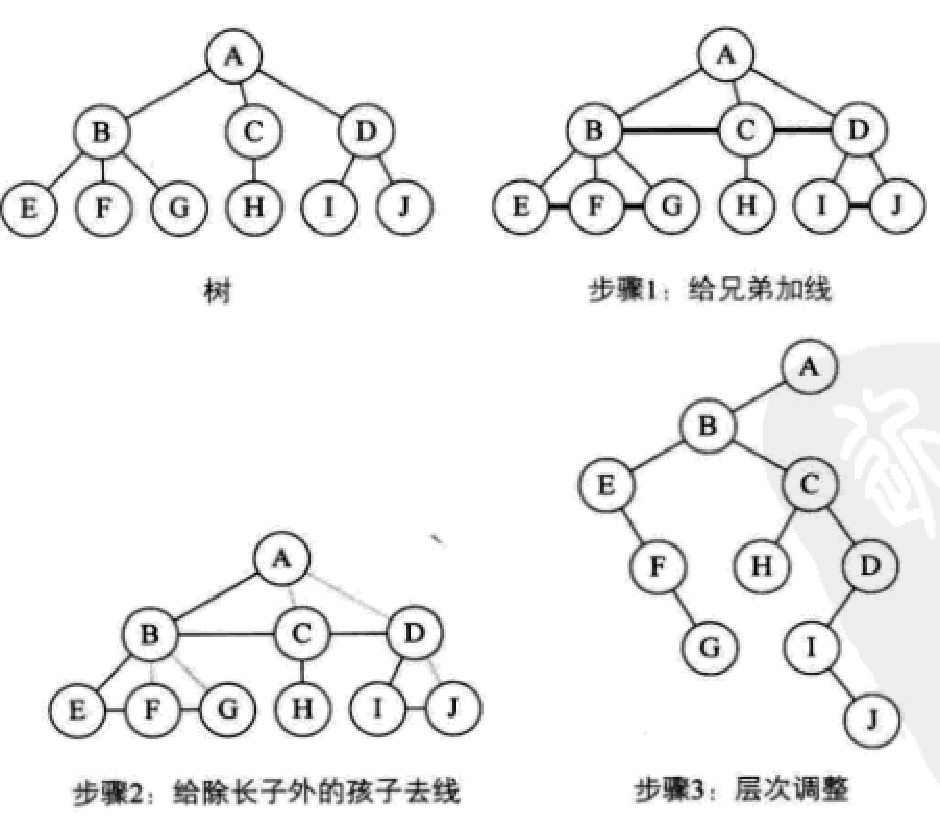
\includegraphics[width=3.5in]{Chapters/Ch05/Fig/tree2bitree.pdf}
  \end{figure}
\end{frame}

\subsubsection{森林转换为二叉树}
\begin{frame}\ft{\subsubsecname}
  步骤:
  \begin{itemize}
  \item[1.]  把每棵树转换为二叉树。\\[0.1in]
  \item[2.]  第一棵二叉树不动,从第二棵二叉树开始,依次把后一棵二叉树的根结点作为前一棵二叉树的根结点的右孩子,用线连接起来。当所有的二叉树连接起来后就得到了由森林转换来的二叉树。
  \end{itemize}
\end{frame}

\begin{frame}\ft{\subsubsecname}
  \begin{figure}
    \centering
    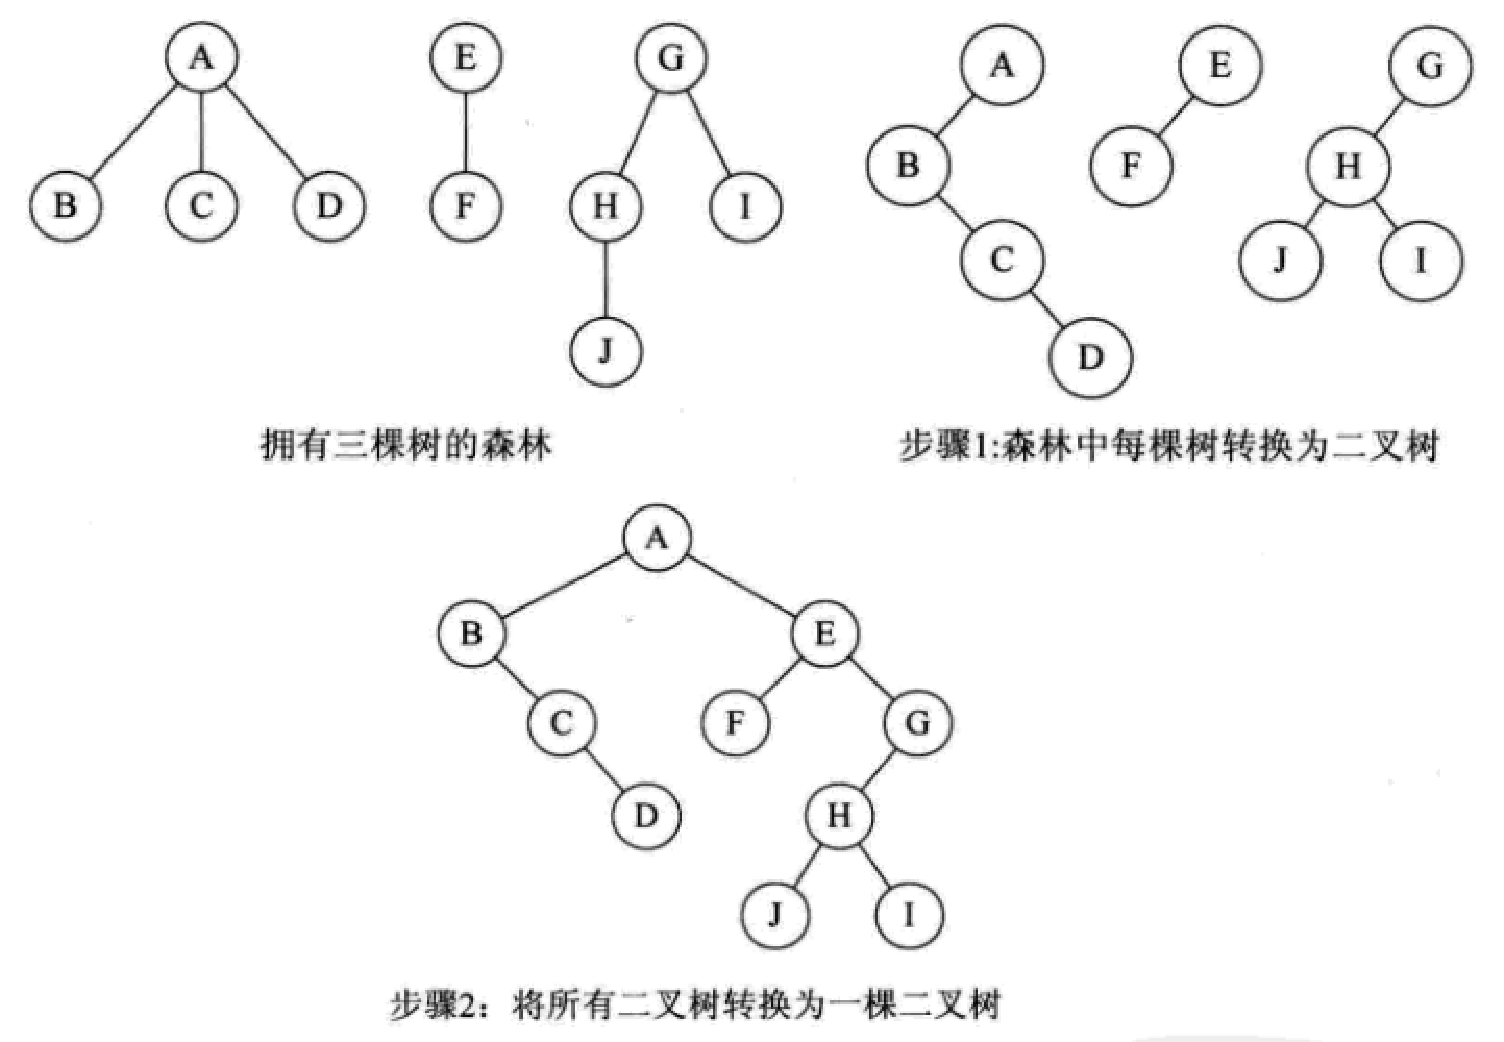
\includegraphics[width=4in]{Chapters/Ch05/Fig/forest2bitree.pdf}
  \end{figure}
\end{frame}


\subsubsection{二叉树转换为树}
\begin{frame}\ft{\subsubsecname}
  步骤:
  \begin{itemize}
  \item[1.]  \blue{加线:}若某结点的左孩子存在,则将这个左孩子的右孩子、右孩子的右孩子、右孩子的右孩子的右孩子、......,即左孩子的$n$个右孩子作为此结点的孩子。将该结点与这些右孩子用线连接起来。\\[0.1in]
  \item[2.]  \blue{去线:}删除原二叉树中所有结点与其右孩子的连线。\\[0.1in] 
  \item[3.]  \blue{层次调整:}使之结构层次分明。
  \end{itemize}
\end{frame}

\begin{frame}\ft{\subsubsecname}
  \begin{figure}
    \centering
    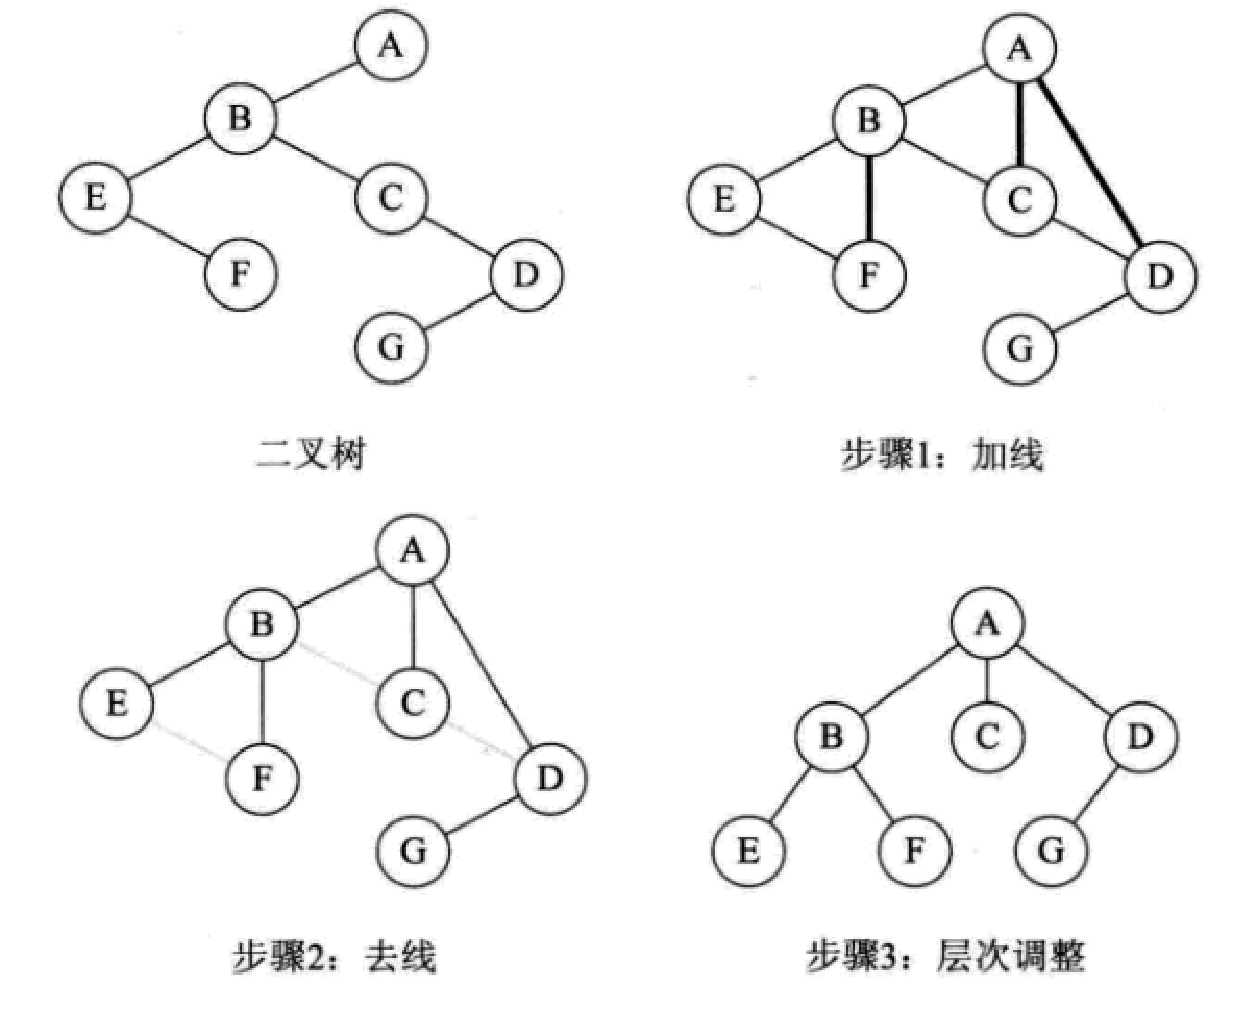
\includegraphics[width=4in]{Chapters/Ch05/Fig/bitree2tree.pdf}
  \end{figure}
\end{frame}

\subsubsection{二叉树转换为森林}
\begin{frame}\ft{\subsubsecname}
  判断一棵二叉树能够转换成一棵树还是森林,只要看这棵二叉树的根结点有没有右孩子,有就是森林,没有就是一棵树。转换成森林的步骤:
  \begin{itemize}
  \item[1.] 从根结点开始,若右孩子存在,则把与右孩子结点的连线删除,再查看分离后的二叉树,若右孩子存在,则连线删除,......,直到所有右孩子连线都删除为止,得到分离的二叉树。\\[0.1in]
  \item[2.] 再将每棵分离后的二叉树转换为树即可。
  \end{itemize}
\end{frame}

\begin{frame}\ft{\subsubsecname}
  \begin{figure}
    \centering
    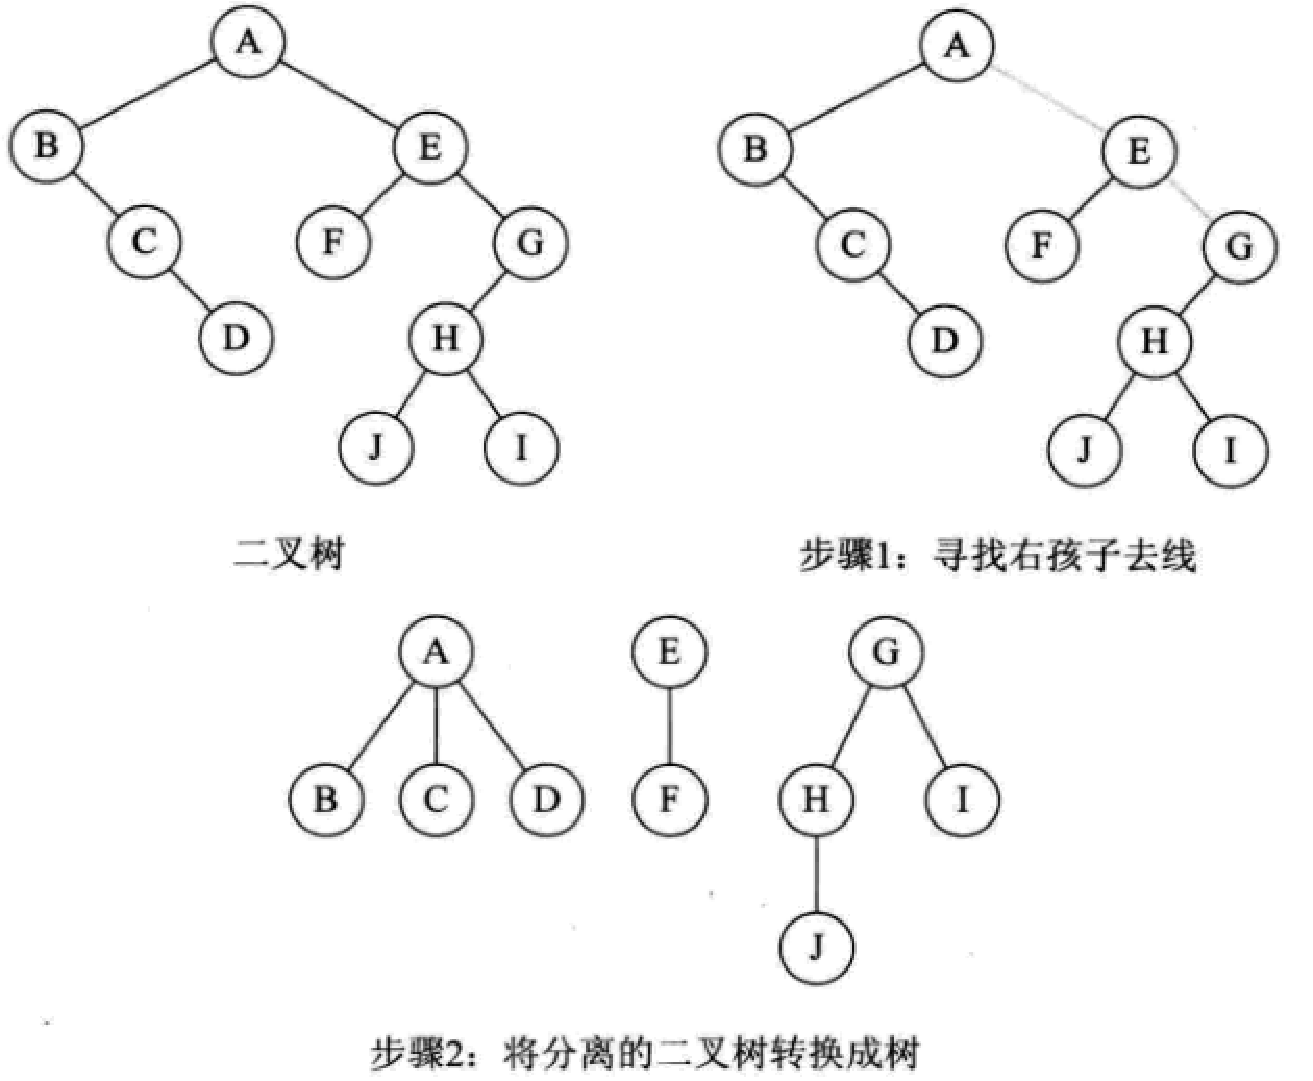
\includegraphics[width=4in]{Chapters/Ch05/Fig/bitree2forest.pdf}
  \end{figure}
\end{frame}

\subsubsection{树和森林的遍历}
\begin{frame}\ft{\subsubsecname}
  树的遍历分为两种方式:
  \begin{itemize}
  \item[1.] \blue{先根遍历:}先访问树的根结点,然后依次先根遍历根的每棵子树。
  \item[2.] \blue{后根遍历:}先依次后根遍历每棵子树,然后再访问根结点。
  \end{itemize}

  %\pause 
  \begin{figure}
    \centering
    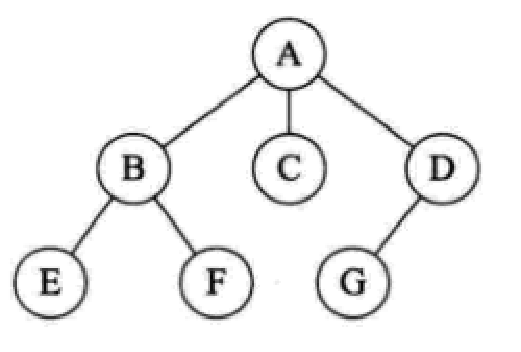
\includegraphics[width=1.8in]{Chapters/Ch05/Fig/tree.pdf}
  \end{figure}

  %\pause 
  \tf先根遍历序列为A、B、E、F、C、D、G;

  \tf后根遍历序列为E、F、B、C、G、D、A。
\end{frame}

\begin{frame}\ft{\subsubsecname}
  森林的遍历也分为两种方式:
  \begin{itemize}
  \item[1.] \blue{前序遍历:}先访问森林中第一棵树的根结点,然后再依次先跟遍历根的每棵子树,再依次用同样方式遍历除去第一棵树的剩余树构成的森林。
  \item[2.] \blue{后序遍历:}先访问森林中第一棵树,后根遍历每棵子树,然后再访问根结点,再依次同样方式遍历除去第一棵树的剩余树构成的森林。
  \end{itemize}

  %\pause 
  \begin{figure}
    \centering
    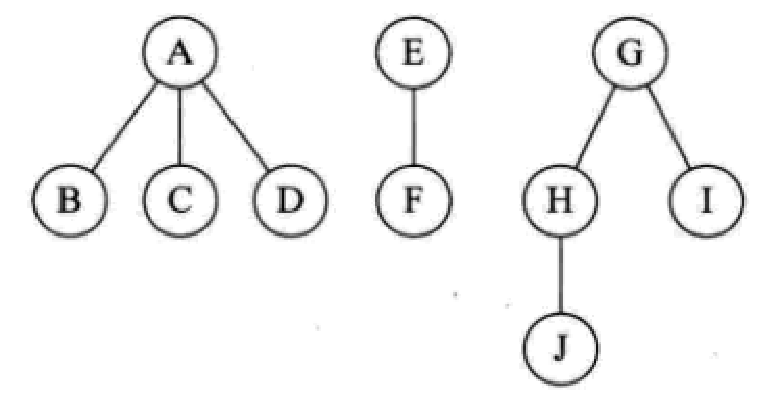
\includegraphics[width=2.5in]{Chapters/Ch05/Fig/forest.pdf}
  \end{figure}

  %\pause 
  \tf先根遍历序列为A、B、C、D、E、F、G、H、J、I;

  \tf后根遍历序列为B、C、D、A、F、E、J、H、G。
\end{frame}

\begin{frame}\ft{\subsubsecname}
  \begin{figure}
    \centering
    \begin{minipage}{0.45\textwidth}
      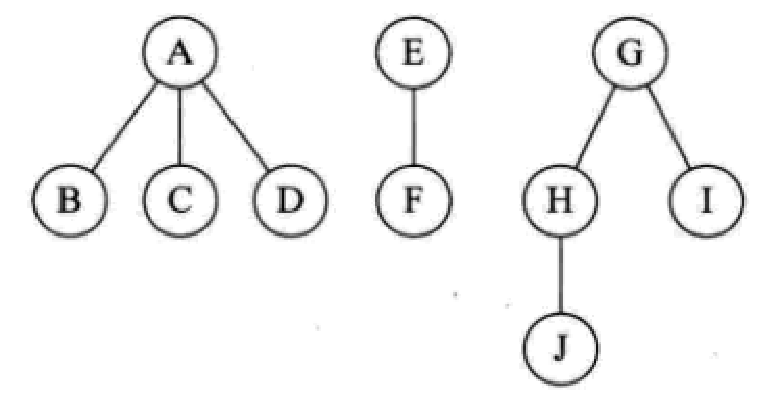
\includegraphics[width=2.2in]{Chapters/Ch05/Fig/forest.pdf}  
    \end{minipage}
    \begin{minipage}{0.45\textwidth}
      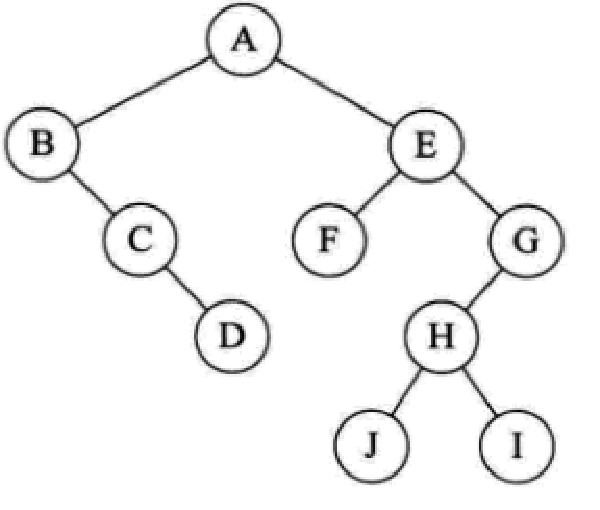
\includegraphics[width=1.6in]{Chapters/Ch05/Fig/bitree.pdf}  
    \end{minipage}    
  \end{figure}
  %\pause 
  \blue{森林的前序遍历和二叉树的前序遍历结果相同,森林的后续遍历和二叉树的中序遍历结果相同。}
\end{frame}



%\section{黑色文字白色背景}
%
%\begin{frame}{简要介绍}
%\mylead{Epyt} 是一个简洁美观的 Beamer 演示主题。它有这些特点:\pause
%\begin{itemize}[<+->]
%\item 结构简洁,只有包含必需元素的底栏,没有顶栏和侧栏。
%\item 内容简洁,列表环境和定理环境可以使用简单形式。
%\item 配色简洁,仅仅用到几种背景色和前景色。
%\end{itemize}
%\end{frame}
%
%\begin{frame}{下载安装}
%\mylead{Epyt} 主题已经包含在主要的 TeX 发行版中。
%\begin{itemize}
%  \item 在 MiKTeX 中作为 \mybold{beamertheme-epyt} 宏包。
%  \item 在 TeXLive 中作为 \mybold{beamertheme-epyt} 宏包。
%\end{itemize}
%你可以在包管理器中安装它。当然也可以直接从
%\href{https://www.ctan.org/pkg/beamertheme-epyt}{CTAN} 中下载并安装。
%\end{frame}
%
%\begin{frame}[fragile]{开始使用}
%要使用 \mylead{epyt} 主题,可以在导言区中加入下面一行。
%\begin{lstlisting}
%\usetheme{epyt}
%\end{lstlisting}\pause
%如果要使用中文,可以添加 \verb ctex 宏包,例如:
%\begin{lstlisting}
%\usepackage[UTF8,noindent]{ctex}
%\end{lstlisting}
%\end{frame}
%
%\begin{frame}[fragile]{样式选用}
%\mylead{Epyt} 主题中包含了多种样式,可以在载入该主题时选用。
%\begin{lstlisting}
%\usetheme[style=gamma]{epyt}
%\end{lstlisting}
%\pause 在文档中间可以用下面命令切换到另一个样式。
%\begin{lstlisting}
%\epytsetup{style=beta}
%\end{lstlisting}
%\end{frame}
%
%\begin{frame}{可用的样式}
%\mylead{Epyt} 主题中所有可用的样式如下所列。
%\begin{description}
%  \item[alpha] 白色文字,黑色背景
%  \item[beta]  黑色文字,白色背景
%  \item[delta] 白色文字,蓝色背景
%  \item[gamma] 白色文字,绿色背景
%  \item[zeta]  白色文字,红色背景
%\end{description}
%\pause
%其中默认样式为 \mybold{beta}。这也是此文档当前正在使用的样式。
%\end{frame}
%
%\begin{frame}{预定义的颜色}
%每种样式都预先定义了五种强调颜色。当前样式的强调颜色如下所示。
%\begin{flushleft}
%\textcolor{acolor1}{acolor1}
%\textcolor{acolor2}{acolor2}
%\textcolor{acolor3}{acolor3}
%\textcolor{acolor4}{acolor4}
%\textcolor{acolor5}{acolor5}
%\end{flushleft}
%\pause 每种样式也预先定义了五种填充颜色,如下所示。
%\begin{flushleft}
%\colorbox{fcolor1}{fcolor1}
%\colorbox{fcolor2}{fcolor2}
%\colorbox{fcolor3}{fcolor3}
%\colorbox{fcolor4}{fcolor4}
%\colorbox{fcolor5}{fcolor5}
%\end{flushleft}
%\pause 用 tikz 绘图时可以使用这些预先定义的颜色。
%\end{frame}
%
%\epytsetup{style=gamma}
%
%\begin{frame}[plain]\transboxout
%\titlepage
%\end{frame}
%
%\section{白色文字绿色背景}
%
%\begin{frame}{预定义的颜色}
%当前样式预先定义了五种强调颜色,如下所示。
%\begin{flushleft}
%\textcolor{acolor1}{acolor1}
%\textcolor{acolor2}{acolor2}
%\textcolor{acolor3}{acolor3}
%\textcolor{acolor4}{acolor4}
%\textcolor{acolor5}{acolor5}
%\end{flushleft}
%当前样式预先定义了五种填充颜色,如下所示。
%\begin{flushleft}
%\colorbox{fcolor1}{fcolor1}
%\colorbox{fcolor2}{fcolor2}
%\colorbox{fcolor3}{fcolor3}
%\colorbox{fcolor4}{fcolor4}
%\colorbox{fcolor5}{fcolor5}
%\end{flushleft}
%\end{frame}
%
%\begin{frame}[fragile]{有序列表}
%无序列表前面已经看到,现在来看看有序列表。一个 Beamer 的主题由下列四部分组成:\pause
%\begin{enumerate}[<+->]
%\item 外部主题,用 \verb!\usebeameroutertheme! 命令;
%\item 内部主题,用 \verb!\usebeamerinnertheme! 命令;
%\item 颜色主题,用 \verb!\usebeamercolortheme! 命令;
%\item 字体主题,用 \verb!\usebeamerfonttheme! 命令。
%\end{enumerate}
%\end{frame}
%
%\epytsetup{style=delta}
%
%\begin{frame}[plain]\transboxout
%\titlepage
%\end{frame}
%
%\section{白色文字蓝色背景}
%
%\begin{frame}{预定义的颜色}
%当前样式预先定义了五种强调颜色,如下所示。
%\begin{flushleft}
%\textcolor{acolor1}{acolor1}
%\textcolor{acolor2}{acolor2}
%\textcolor{acolor3}{acolor3}
%\textcolor{acolor4}{acolor4}
%\textcolor{acolor5}{acolor5}
%\end{flushleft}
%当前样式预先定义了五种填充颜色,如下所示。
%\begin{flushleft}
%\colorbox{fcolor1}{fcolor1}
%\colorbox{fcolor2}{fcolor2}
%\colorbox{fcolor3}{fcolor3}
%\colorbox{fcolor4}{fcolor4}
%\colorbox{fcolor5}{fcolor5}
%\end{flushleft}
%\end{frame}
%
%\epytsetup{style=alpha}
%
%\begin{frame}[plain]\transboxout
%\titlepage
%\end{frame}
%
%\section{白色文字黑色背景}
%
%\begin{frame}{预定义的颜色}
%当前样式预先定义了五种强调颜色,如下所示。
%\begin{flushleft}
%\textcolor{acolor1}{acolor1}
%\textcolor{acolor2}{acolor2}
%\textcolor{acolor3}{acolor3}
%\textcolor{acolor4}{acolor4}
%\textcolor{acolor5}{acolor5}
%\end{flushleft}
%当前样式预先定义了五种填充颜色,如下所示。
%\begin{flushleft}
%\colorbox{fcolor1}{fcolor1}
%\colorbox{fcolor2}{fcolor2}
%\colorbox{fcolor3}{fcolor3}
%\colorbox{fcolor4}{fcolor4}
%\colorbox{fcolor5}{fcolor5}
%\end{flushleft}
%\end{frame}
%
%\begin{frame}{例子证明}
%\begin{example}
%证明当$x>0$时不等式$\mathrm{e}^x>1+x$成立。
%\end{example}\pause
%\begin{proof}
%令$f(x)=\mathrm{e}^x-x-1$。则当$x>0$时有
%$$f'(x)=\mathrm{e}^x-1>0.$$
%因此,当$x>0$时$f(x)>f(0)=0$。得证。
%\end{proof}
%\end{frame}
%
%\epytsetup{style=zeta}
%
%\begin{frame}[plain]\transboxout
%\titlepage
%\end{frame}
%
%\section{白色文字红色背景}
%
%\begin{frame}{预定义的颜色}
%当前样式预先定义了五种强调颜色,如下所示。
%\begin{flushleft}
%\textcolor{acolor1}{acolor1}
%\textcolor{acolor2}{acolor2}
%\textcolor{acolor3}{acolor3}
%\textcolor{acolor4}{acolor4}
%\textcolor{acolor5}{acolor5}
%\end{flushleft}
%当前样式预先定义了五种填充颜色,如下所示。
%\begin{flushleft}
%\colorbox{fcolor1}{fcolor1}
%\colorbox{fcolor2}{fcolor2}
%\colorbox{fcolor3}{fcolor3}
%\colorbox{fcolor4}{fcolor4}
%\colorbox{fcolor5}{fcolor5}
%\end{flushleft}
%\end{frame}

\end{document}
